%%%%%%%%%%%%%%%%%%%%%%%%%%%%%%%%%%%%%%%%%
% Stylish Article
% LaTeX Template
% Version 2.1 (1/10/15)
%
% This template has been downloaded from:
% http://www.LaTeXTemplates.com
%
% Original author:
% Mathias Legrand (legrand.mathias@gmail.com) 
% With extensive modifications by:
% Vel (vel@latextemplates.com)
%
% License:
% CC BY-NC-SA 3.0 (http://creativecommons.org/licenses/by-nc-sa/3.0/)
%
%%%%%%%%%%%%%%%%%%%%%%%%%%%%%%%%%%%%%%%%%

%----------------------------------------------------------------------------------------
%	PACKAGES AND OTHER DOCUMENT CONFIGURATIONS
%----------------------------------------------------------------------------------------

\documentclass[10pt]{SelfArx} % Document font size and equations flushed left
\usepackage[scaled]{helvet}
\renewcommand\familydefault{\sfdefault} 
\usepackage[T1]{fontenc}

\usepackage[english]{babel} % Specify a different language here - english by default

\usepackage{lipsum} % Required to insert dummy text. To be removed otherwise
\usepackage{subfig}
\usepackage{amsmath}
\usepackage{afterpage}
\DeclareMathOperator{\Var}{Var}
\newcommand{\pder}[2][]{\frac{\partial#1}{\partial#2}}
\newcommand{\ppder}[2][]{\frac{\partial^2#1}{\partial#2^2}}
\usepackage{amsthm}
\usepackage[nice]{nicefrac}
\theoremstyle{definition}
\newtheorem{exmp}{Example}[section]

\usepackage{algorithm}% http://ctan.org/pkg/algorithms
\usepackage{algpseudocode}% http://ctan.org/pkg/algorithmicx


%------------------------
%   EXAMPLE USES OF STYLES
%--------------

%\begin{figure*}[ht]\centering % Using \begin{figure*} makes the figure take up the entire width of the page
%\includegraphics[width=\linewidth]{view}
%\caption{Wide Picture}
%\label{fig:view}
%\end{figure*}


%\begin{enumerate}[noitemsep] % [noitemsep] removes whitespace between the items for a compact look
%\item First item in a list
%\item Second item in a list
%\item Third item in a list
%\end{enumerate}



%\paragraph{Paragraph} \lipsum[7] % Dummy text
%\paragraph{Paragraph} \lipsum[8] % Dummy text


%\begin{table}[hbt]
%\caption{Table of Grades}
%\centering
%\begin{tabular}{llr}
%\toprule
%\multicolumn{2}{c}{Name} \\
%\cmidrule(r){1-2}
%First name & Last Name & Grade \\
%\midrule
%John & Doe & $7.5$ \\
%Richard & Miles & $2$ \\
%\bottomrule
%\end{tabular}
%\label{tab:label}
%\end{table}

%\begin{description}
%\item[Word] Definition
%\item[Concept] Explanation
%\item[Idea] Text
%\end{description}


%\begin{itemize}[noitemsep] % [noitemsep] removes whitespace between the items for a compact look
%\item First item in a list
%\item Second item in a list
%\item Third item in a list
%\end{itemize}




%----------------------------------------------------------------------------------------
%	COLUMNS
%----------------------------------------------------------------------------------------

\setlength{\columnsep}{0.55cm} % Distance between the two columns of text
\setlength{\fboxrule}{0.75pt} % Width of the border around the abstract

%----------------------------------------------------------------------------------------
%	COLORS
%----------------------------------------------------------------------------------------

\definecolor{color1}{RGB}{0,0,90} % Color of the article title and sections
\definecolor{color2}{RGB}{0,20,20} % Color of the boxes behind the abstract and headings

%----------------------------------------------------------------------------------------
%	HYPERLINKS
%----------------------------------------------------------------------------------------

\usepackage{hyperref} % Required for hyperlinks
\hypersetup{hidelinks,colorlinks,breaklinks=true,urlcolor=color2,citecolor=color1,linkcolor=color1,bookmarksopen=false,pdftitle={Title},pdfauthor={Author}}
\usepackage[capitalise]{cleveref}

\crefname{exmp}{example}{examples}
\Crefname{exmp}{Example}{Examples}
%----------------------------------------------------------------------------------------
%	ARTICLE INFORMATION
%----------------------------------------------------------------------------------------

\JournalInfo{Internship report for the Instituto Colombia del Petróleo (ICP)} % Journal information
\Archive{In requirement of the degree Master of science Applied Physics, TU Delft, the Netherlands} % Additional notes (e.g. copyright, DOI, review/research article)

\PaperTitle{A general recipe for obtaining adjoint equations and gradients and its application to full waveform inversion of 2D isotropic elastic media in finite difference time-domain} % Article title
\PageHeading{ICP - CPS}

\Authors{J. J. Wesdorp*} % Authors

\Keywords{ Herling Gonzalez-Alvarez \textsuperscript{1} \newline Prof. Koen van Dongen \textsuperscript{2} \newline Prof. Ana Ramirez \textsuperscript{3}} % Keywords - if you don't want any simply remove all the text between the curly brackets
\newcommand{\keywordname}{Supervisors} % Defines the keywords heading name
\affiliation{\textsuperscript{1}\textit{Instituto Colombia del Petróleo (ICP), Piedecuesta, Colombia}} % Author affiliation
\affiliation{\textsuperscript{2}\textit{Technical University of Delft, the Netherlands}} % Author affiliation
\affiliation{\textsuperscript{3}\textit{Universidad Industrial de Santander (UIS), CPS research group, Bucaramanga, Colombia}}
\affiliation{*\textbf{email}: jaapwesdorp@gmail.com} % Corresponding author
%----------------------------------------------------------------------------------------
%	ABSTRACT
%----------------------------------------------------------------------------------------

\Abstract{\lipsum[1]~}

%----------------------------------------------------------------------------------------

\begin{document}

\flushbottom % Makes all text pages the same height

\maketitle % Print the title and abstract box

\onecolumn

\tableofcontents % Print the contents section

\thispagestyle{empty} % Removes page numbering from the first page
%----------------------------------------------------------------------------------------
%	ARTICLE CONTENTS
%----------------------------------------------------------------------------------------

\section{Introduction} % The \section*{} command stops section numbering
Full waveform inversion can be used a tool to quantitatively image material properties of the earth, or tissue. 

30 years ago -> ~\cite{Tarantola1986} proposed FWI. Now since 10 years the industry is making use of FWI in their processing workflow due to the gain in computing power.

Initially mostly acoustic, but there is interest in modeling elastic waves, since you can see phenomena like: groundroll waves, surface waves ->(WHAT ELSE IS SPECIAL ABOUT ELASTIC). 

FWI requires one to know the gradient of your guessed model with respect to measured shots, therefore the \emph{adjoint state method}~\cite{Plessix2006} makes this a lot more efficient. 

This research was performed as part of an internship for the Instituto Colombia del Petróleo (ICP). The first goal was to model the isotropic 2D elastic wave equation, which is described in section ...
The second goal was to find the adjoint operator and gradients for the elastic case. Since no explicit declaration is given yet for the elastic case in current literature and the adjoint state method is usually described in a very abstract way, this work shows an "engineers approach" to obtaining the adjoint system and gradient expressions for any general set of equations in sec .... This method is applied to the elastic case in sec ..., and more exampĺes are given in~\cref{sec:examples}.
This method is subsequently tested by performing FWI on a test model described in sec ...



%\addcontentsline{toc}{section}{Introduction} % Adds this section to the table of contents

%-------------------------------------------------------------------------------------------------------------------

\section{A simple recipe for the adjoint state method}


\subsection{Adjoint method for general discretized linear systems}\label{sec:discretized_math}
This section shows in simple steps how to obtain the adjoint equations and gradients given a general system of wave equations and initial and boundary conditions of zero. These are cast in a general form usually present in acoustic, elastic or electromagnetic FWI applications. The proof of validity and derivation of this method is presented in \cref{sec:general_math} for an more general set of equations based on the notes of Bradley\cite{Bradley2012}.
\subsubsection{Formulation}{}
Say we have a model representing the earth (in seismic applications) or tissue (in medical applications) for some parameter like density $\rho$ or speed of sound $v$, which we discretized in a grid in space into $N_g  (= N_x \times N_z$ in 2D) points. If we want to model $d_m$ parameters over this grid we can write the values of these parameters over the grid as a vector $\vec{m}$ of dimension $d_m \times N_g$. We want to model $d_s$ fields also discretized in space on the same grid we can write them as a vector $\vec{s}$ of dimension $d_s \times N_g$. Any FWI problem of wave equations(e.g electromagnetic, elastic or acoustic), whether they are  multiple first or second order PDE's in time and space, can be written as the following minimization problem given a set of discretized(only in space) ODEs
\begin{equation}
\label{eq:discretised_linear_system}
\begin{aligned}
\underset{\vec{m}}{\text{min}}\  & \chi\left(\vec{s},\vec{m}\right) =   \int_0^T f\left(\vec{s},\vec{m}\right) dt \\
\text{subject to}\ \ \   &   T\left(\vec{m}\right)\ddot{\vec{s}} - C\left(\vec{m}\right)\dot{\vec{s}} - A\left(\vec{m}\right)\vec{s} -\vec{b}\left(\vec{m}\right)= 0 \\
 \text{with B.C}\ \ \  &  \vec{s}\left(0\right)  = 0 \\
 &  \dot{\vec{s}}\left(0\right)  = 0 \\
\end{aligned}
\end{equation}
where $T, C, A$ are big matrices of $(N_g \times d_s) \times (N_g \times d_s)$ coefficients which follow from the discretization in space of a PDE system, $\vec{b}\left(\vec{m}\right)$ is a vector of the same length of $\vec{s}$ which contains the source terms, $\chi$ denotes the total cost function and we denote time explicitely by taking the integral of some function $f$ since usually we simplify each cost function into this form. 

\subsubsection{Gradients and adjoint}
The goal of the adjoint state method is avoiding the calculation of the Frechet derivatives $\pder{\chi}{m}$ since they require the amount of forward modeling evaluations to scale with the grid size of the model. We can apply~\cref{eq:general_gradient} of~\cref{sec:general_math} to the system of~\cref{eq:discretised_linear_system} and find the following simpler expression for the total gradient with respect to \emph{all} model parameters
\begin{equation}\label{eq:gradient_discretised_linear}
\frac{d\chi}{d\vec{m}} = \int_0^T \pder[f]{\vec{m}} + \vec{\lambda}^T \left(\pder[T]{\vec{m}}\ddot{\vec{s}} - \pder[C]{\vec{m}}\dot{\vec{s}} - \pder[A]{\vec{m}}\vec{s} -\pder[b]{\vec{m}}\right) dt
\end{equation}
Note that the gradients $\pder[T]{\vec{m}}, \pder[C]{\vec{m}}, \pder[A]{\vec{m}}$ can be seen as a sum of all the $3N$ derivatives of each component of the matrices $T\left(\vec{m}\right), C\left(\vec{m}\right), A\left(\vec{m}\right)$ to the discrete variables $\vec{m}_i$, but in practice we can write this into simple compact expressions as shown in the examples in~\cref{sec:examples}.
The adjoint variable $\lambda$ is given using~\cref{eq:general_adjoint} and applying it to our system of~\cref{eq:discretised_linear_system} we obtain
\begin{equation}\label{eq:adjoint_discretised_linear}
T^T\left(\vec{m}\right) \ddot{\vec{\lambda}} = -C^T\left(\vec{m}\right)\dot{\vec{\lambda}} + A^T\left(\vec{m}\right) \vec{\lambda} - \pder[f]{\vec{s}}
\end{equation}
giving an extra set of equations that need to be solved. 


\subsubsection{Least squares cost function}
In most cases the cost function is given by the misfit between observed data $d$ at certain receiver positions $y_R$ and the modeled data at the same positions $s_{y_R}$, so $f\left(\vec{s}\right)$ is given by 
\begin{equation}\label{eq:cost_function_standard}
f\left(\vec{s}\right) =\frac{1}{2} \sum_{R}^{N_R}||s_{y_R} - d_{y_R}||^2
\end{equation}
where the sum goes over all receiver positions. Note that $f\left(\vec{s}\right)$ does not depend directly on the model parameters $\vec{m}$ making the gradient expression simpler since $\pder[f]{\vec{m}} = 0$. We thus obtain
\begin{equation}\label{eq:adjoint_source}
\pder[f]{\vec{s}} =  \sum_{R}^{N_R}s_{y_R} - d_{y_R} 
\end{equation}
which are the well known residuals injected as a source for the adjoint equations. 


\subsection{Adjoint and gradients of the elastic wave equation}
Elastic waves in 2D isotropic media can be modeled by using only three parameters, the density $\rho$ and the two Lame parameters $\mu, \lambda$ and follow the following system of equations
\begin{equation}\label{eq:elastic_system}
\begin{aligned}
\rho \pder[v_x]{t} = \pder[\tau_{xx}]{x} + \pder[\tau_{xz}]{z} \\
\rho \pder[v_z]{t} = \pder[\tau_{xz}]{x} + \pder[\tau_{zz}]{z} \\
\pder[\tau_{xx}]{t} = \left(\lambda + 2\mu\right) \pder[v_x]{x} + \lambda \pder[v_z]{z} + b_{xx} \\
\pder[\tau_{zz}]{t} = \left(\lambda + 2\mu\right) \pder[v_z]{z} + \lambda \pder[v_x]{x} + b_{zz} \\
\pder[\tau_{xz}]{t} = \mu\left( \pder[v_x]{z} + \pder[v_z]{x}\right) \\
\end{aligned}
\end{equation} 
where we only added the source to the stress as to resemble an earthquake. The form of $b$ is independent of the model parameters and usually taken as a ricker wavelet. 
writing this in the form of~\cref{eq:discretised_linear_system} gives 
\begin{equation}
T(m) = 0,\ 
s = 
\begin{bmatrix}
v_x \\
v_z \\
\tau_{xx}\\
\tau_{zz} \\
\tau_{xz} \\
\end{bmatrix},\ C\left(m\right) = -
\begin{bmatrix}
\rho & 0 & 0 & 0 & 0 \\
0 & \rho & 0 & 0 & 0 \\
0 & 0 & 1 & 0 & 0 \\
0 & 0 & 0 & 1 & 0 \\
0 & 0 & 0 & 0 & 1 \\
\end{bmatrix}
\end{equation}
and 
\begin{equation}
A\left(m\right) = 
\begin{bmatrix}
0 & 0 & \mathcal{D}_x & 0 & \mathcal{D}_z \\
0 & 0 & 0 & \mathcal{D}_z & \mathcal{D}_x \\
\left(\lambda + 2\mu\right)\mathcal{D}_x & \lambda \mathcal{D}_z & 0 & 0 & 0 \\
\lambda \mathcal{D}_x & \left(\lambda + 2\mu\right) \mathcal{D}_z & 0 & 0 & 0 \\
\mu \mathcal{D}_z & \mu \mathcal{D}_x & 0 & 0 & 0 \\
\end{bmatrix}
\end{equation}
Thus we have $C^T\left(m\right) = C\left(m\right)$ and 
\begin{equation}
A^T\left(m\right) = 
\begin{bmatrix}
0 & 0 & -\mathcal{D}_x\left(\lambda + 2\mu\right) & -\mathcal{D}_x\lambda & -\mathcal{D}_z\mu \\
0 & 0 & -\mathcal{D}_z \lambda & -\mathcal{D}_z\left(\lambda + 2\mu\right) & -\mathcal{D}_x\mu \\
-\mathcal{D}_x & 0 & 0 & 0 & 0 \\
0 & -\mathcal{D}_z & 0 & 0 & 0 \\
-\mathcal{D}_z & -\mathcal{D}_x & 0 & 0 & 0 \\
\end{bmatrix}
\end{equation}
which in turn (when transforming back to the continuous domain from the discrete variables) results in the following adjoint equations(naming the adjoint variable $l$) as defined in~\cref{eq:adjoint_discretised_linear}
\begin{equation}\label{eq:elastic_adjoint}
\begin{aligned}
\rho \pder[l_1]{t} &= \pder[\left(\left(\lambda + 2\mu\right)l_3\right)]{x} + \pder[\left(\lambda l_4\right)]{x} + \pder[\left(\mu \lambda_5\right)]{z} \\
\rho \pder[l_2]{t} &= \pder[\left(\lambda l_3\right)]{z} + \pder[\left(\left(\lambda + 2\mu\right)l_4\right)]{z} + \pder[\left(\mu \lambda_5\right)]{x} \\
\pder[l_3]{t} &= \pder[l_1]{x}\\
\pder[l_4]{t} &= \pder[l_2]{z}\\
\pder[l_5]{t} &= \pder[l_1]{z} + \pder[l_2]{x}\\
\end{aligned}
\end{equation}
where the order of differentiation and multiplication with the model parameters is important. 
The gradients then follow from~\cref{eq:gradient_discretised_linear}, giving 

\begin{equation}
\begin{aligned}
\frac{d\chi}{d\rho} &= \int_0^T - l^T \pder[C]{\rho} \dot s\ dt \\
&=\int_0^T
 \begin{bmatrix}
\vec{l_1}&\vec{l_2}&\vec{l_3} &\vec{l_4} & \vec{l_5}\\
\end{bmatrix}
 \begin{bmatrix}
I & 0 & 0 & 0 & 0 \\
0  & I & 0&0&0\\
0 & 0 & 0&0&0\\
0&0&0&0&0\\
0&0&0&0&0
\end{bmatrix}
\begin{bmatrix}
\vec{\dot{v_x}}\\
\vec{\dot{v_y}}\\
\vec{\dot{\tau_{xx}}}\\
\vec{\dot{\tau_{zz}}}\\
\vec{\dot{\tau_{xz}}}
\end{bmatrix} \\
&=\int_0^T \vec{l_1}\vec{\dot{v}}_x + \vec{l_2}\vec{\dot{v}}_z \ dt 
\end{aligned}
\end{equation},

\begin{equation}
\begin{aligned}
\frac{d\chi}{d\lambda} &= \int_0^T - l^T \pder[A]{\lambda} s\ dt \\
&=-\int_0^T
 \begin{bmatrix}
\vec{l_1}&\vec{l_2}&\vec{l_3} &\vec{l_4} & \vec{l_5}\\
\end{bmatrix}
 \begin{bmatrix}
0 & 0 & 0 & 0 & 0 \\
0  & 0 & 0&0&0\\
\mathcal{D}_x & \mathcal{D}_z & 0&0&0\\
\mathcal{D}_x&\mathcal{D}_z&0&0&0\\
0&0&0&0&0
\end{bmatrix}
\begin{bmatrix}
\vec{{v_x}}\\
\vec{{v_y}}\\
\vec{{\tau_{xx}}}\\
\vec{{\tau_{zz}}}\\
\vec{{\tau_{xz}}}
\end{bmatrix} \\
&=-\int_0^T \left(\vec{l_3} + \vec{l_4}\right) \left(\pder[\vec{v_x}]{x} + \pder[\vec{v_z}]{z}\right) 
\end{aligned}
\end{equation} and

\begin{equation}
\begin{aligned}
\frac{d\chi}{d\mu} &= \int_0^T - l^T \pder[A]{\mu} s\ dt \\
&=-\int_0^T
 \begin{bmatrix}
\vec{l_1}&\vec{l_2}&\vec{l_3} &\vec{l_4} & \vec{l_5}\\
\end{bmatrix}
 \begin{bmatrix}
0 & 0 & 0 & 0 & 0 \\
0  & 0 & 0&0&0\\
2\mathcal{D}_x & 0 & 0&0&0\\
0 &2\mathcal{D}_z&0&0&0\\
\mathcal{D}_z&\mathcal{D}_x&0&0&0
\end{bmatrix}
\begin{bmatrix}
\vec{{v_x}}\\
\vec{{v_y}}\\
\vec{{\tau_{xx}}}\\
\vec{{\tau_{zz}}}\\
\vec{{\tau_{xz}}}
\end{bmatrix} \\{}
&=-\int_0^T 2\vec{l_3} \pder[\vec{v_x}]{x} + 2\vec{l_4} \pder[\vec{v_z}]{z} + \vec{l_5}\left(\pder[\vec{v_x}]{z} + \pder[\vec{v_z}]{x}\right) \ dt
\end{aligned}
\end{equation}

%-------------------------------------------------------------------------------------------------------------------

\section{Numerical implementation of the elastic wave equation}
Chapter intro here

\subsection{Staggered grid discrete equations}
We now show the modeling of~\cref{eq:elastic_system}.
Due to the nature of the equations, if we would implement every field at the same grid point in time and space using centered finite differences, we would get decoupling between the velocity and stress in time and space(e.g $V_x$ at time t depending on $\tau$ at time $t \pm \frac{dt}{2}$ which we do not have defined).
This could be solved by using a two times finer grid, but can be more elegantly solved by use a staggered grid following~\cite{Virieux1984}.
Using the notation $\left\{v_x, v_z, \tau_{xx}, \tau_{zz}, \tau_{xz}\right\} = \left\{U, V, X, Z, T \right\}$ we do a "leapfrog" scheme, which in each timestep loops over the spatial directions for calculating $U^{n+\frac{1}{2}},V^{n+\frac{1}{2}}$ as a function of the previously calculated $X^n, Z^n, T^n$ first and consecutively loops over the spatial directions again to calculate $X^{n+1}, Z^{n+1}, T^{n+1}$ depending on the just calculated $U^{n+\frac{1}{2}},V^{n+\frac{1}{2}}$. 
This avoids the decoupling mentioned above, but requires the fields to be defined in different points in the grid.
The numerical equations are then given by (using a 2nd order central difference in time and arbitrary difference operator in space)

\begin{equation}
\left\{
\begin{aligned}
U_{i,j}^{n+\frac{1}{2}}  &= U_{i,j}^{n-\frac{1}{2}} + \frac{\Delta t}{\rho_{i,j}}\left[ D_xX_{i,j}^n + D_zT^n_{i,j}\right] \\
V_{i+\frac{1}{2},j+\frac{1}{2}}^{n+\frac{1}{2}}  &= V_{i+\frac{1}{2},j+\frac{1}{2}}^{n-\frac{1}{2}} + \frac{\Delta t}{\rho_{i+\frac{1}{2},j+\frac{1}{2}}}\left[ D_xT_{i+\frac{1}{2},j+\frac{1}{2}}^n + D_zZ^n_{i+\frac{1}{2},j+\frac{1}{2}}\right] \\
X_{i+\frac{1}{2},j}^{n+1}  &= X_{i+\frac{1}{2},j}^{n} + \Delta t\left[ \left(\lambda_{i+\frac{1}{2},j} + 2 \mu_{i+\frac{1}{2},j}\right)D_xU_{i+\frac{1}{2},j}^{n+\frac{1}{2}} + \lambda_{i+\frac{1}{2},j} D_zV^{n+\frac{1}{2}}_{i+\frac{1}{2},j}\right] \\
Z_{i+\frac{1}{2},j}^{n+1}  &= Z_{i+\frac{1}{2},j}^{n} + \Delta t\left[ \left(\lambda_{i+\frac{1}{2},j} + 2 \mu_{i+\frac{1}{2},j}\right)D_zV_{i+\frac{1}{2},j}^{n+\frac{1}{2}} + \lambda_{i+\frac{1}{2},j} D_xU^{n+\frac{1}{2}}_{i+\frac{1}{2},j}\right] \\
T_{i,j+\frac{1}{2}}^{n+1}  &= T_{i,j+\frac{1}{2}}^{n} + \mu_{i,j+\frac{1}{2}}\Delta t\left[ D_zU_{i,j+\frac{1}{2}}^{n+\frac{1}{2}} + D_xV^{n+\frac{1}{2}}_{i,j+\frac{1}{2}}\right] \\
\end{aligned}\right.
\end{equation}
where for the simplest second order differential operator $D_x A^n_{i,j} = \frac{A^n_{i+\frac{1}{2},j} - A^n_{i-\frac{1}{2},j}}{\Delta_x}$ and $D_z A^n_{i,j} = \frac{A^n_{i,j+\frac{1}{2}} - A^n_{i,j-\frac{1}{2}}}{\Delta_z}$. $n$ denotes the discrete time step, $i,j$ the $x,z$ coordinates respectively, and $\Delta t, \Delta x, \Delta z$ are the stepsizes taken into each direction respectively.
In~\cref{fig:staggered_grid} the staggered grid is shown schematically together with a table to explain the index translations used to transform from the actual implementation to the discrete equations shown above. 
\begin{figure}[hbt]
\caption{(a) Schematic of the staggered grid. The square indicates the position of the velocity field $U$, the diamond that of $V$, the triangle that of $X,Z$ and the upside down triangle that of $T$. Blue indicates that the field is evaluated at time $n+1/2$ and red at time $n$. (b) Table of the staggered grid computational array index conversion. Shows how the 2D computational array indexes for the field arrays are transformed for the staggered grid. For example: if we access array element $V[i,j]$ in the code we obtain the field $v_z$ at real position $i+1/2, j+1/2$ in the grid.}
\label{fig:staggered_grid}
\vspace{5pt}
\centering
\subfloat[][]{
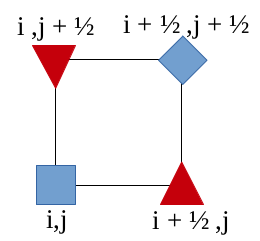
\includegraphics[width=0.25\textwidth]{fig/staggered_grid.png}
}
\qquad
\subfloat[][]{
 \vspace{0pt}
    \centering
    \begin{tabular}{lrr}
    \toprule
    Field & index i transform & index j transform \\
    \midrule
    $U (v_x)$ & $i$ & $j$ \\
    $V (v_z)$ & $i + 1/2$ & $j + 1/2$ \\
    $X (\tau_{xx})$ & $i + 1/2$ & $j$ \\
    $Z (\tau_{zz})$ & $i + 1/2$ & $j$ \\
    $T (\tau_{xz})$ & $i$ & $j + 1/2$ \\

    \bottomrule
    \end{tabular}
     \vspace{0pt}
    \label{tab:label}
}

\end{figure}

\afterpage{
\begin{figure}[p]\centering % Using \begin{figure*} makes the figure take up the entire width of the page
\includegraphics[width=0.8\linewidth]{"fig/field_vx"}
\includegraphics[width=0.8\linewidth]{"fig/field_vx_cpml"}
\caption{Elastic wave propagation in homogeneous media. Top 4 images show the simulation with reflecting boundary conditions and the bottom four with CPML active, giving a clear decrease in reflection amplitude. $V_p=2500$m/s, $V_s=430$m/s, $\rho=1750$m/s, $f_{source}=10$Hz, $n_x=n_z=220$, $d_x=d_z=10$m, $dt=0.3$ms}
\label{fig:sim_homogeneous_cpml}
\end{figure}
\clearpage
}
\subsection{Ricker wavelet source function}
We used a source of the form
\begin{equation}
f\left(t\right) = \left(1 - 2\pi^2 f_q^2 (t-t_0)^2\right) e^{-\pi^2f_q^2 (t-t_0)^2}
\end{equation}
where $f_q$ is the desired center source frequency, $t_0$ the time offset (taken as $\frac{1}{f_q}$ usually). Note that $t_0$ is important since if you start with a non-zero source the FD modeling will become unstable. The source was added equally to both the horizontal and vertical stress $\tau_{xx}$ and $\tau_{zz}$ at each timestep.
\subsection{CPML Absorbing boundaries}
In most seismic cases we have an infinite domain of our model, but we are just interested in a specific part of this domain. In order to simulate only this part without reflecting boundaries one needs to simulate "open" boundaries.
This is performed using Perfectly Matched Layers(PML)~\cite{Berenger1994}. Simply stated PML can be seen as adding as changing the coordinates to complex values in the boundary layers of the grid in which the wave travels, this then exponentially dampens any plane wave traveling through the boundary layer of which the strength depends on the incidence angle, damping less for grazing incidence. Another property of PML is that the reflection coefficient is exactly zero for all incident angles before discretization. The original PML required to extra fields in time, so therefore the Convolutionary PML was introduced(CPML)~\cite{Roden2000}, which allows for the use of memory variables to keep a memory efficient solution and finally and improved version of CPML was introduced to decrease the reflections at grazing incidence angles at the cost of adding extra tunable parameters~\cite{Komatitsch2007}. 

CPML can be easily implemented, since all one needs to do is replace all the finite difference operations on the fields inside the CPML layer by CPML damped variant. This is performed by adding so called memory variables which have their own simple governing differential equations. For the field $K\in\{U,V,X,Z,T\}$ and derivative direction $s\in\{x,z\}$ this becomes
\begin{equation}
D_sK^n_{i,j} \rightarrow \frac{D_sK^n_{i,j}}{\kappa_s} + M_{D_sK|i,j}^n
\end{equation}
where $\kappa_s$ is usually taken as 1 and the memory variable is updated each timestep by
\begin{equation}
     M_{D_sK|i,j}^n = b_s M_{D_sK|i,j}^{n-1} + a_s D_sK^n_{i,j}
\end{equation} 
the damping coefficients $a_s, b_s$ are given by the following formulas
\begin{equation}
\left\{
\begin{aligned}
a_s &= \frac{d_s}{d_s + \alpha_s}\left(b_s - 1\right) \\
b_s &= e ^ {-(d_s + \alpha_s)\Delta t}
\end{aligned}\right.
\end{equation}
where all parameters are chosen following~\cite{Komatitsch2007}. They pick $\alpha_s$ a linearly varying from $\alpha_{max}=\pi f_0$ in the entry of the CPML layer to 0 at the end of the layer and $f_0$ is the center source frequency. $d_s = d_0\left(\frac{\Delta_{cpml} s}{L}\right)^N$ where $\Delta_{cpml} s$ Is the amount of meters inside the CPML layer in direction $s$, $L$ is the total length of the CPML layer (usually taken as the length of 10 grid points), N is the damping order (taken as 2)~\cite{Collino2001}, $d_0$ is given by $d_0=-\left(N +1\right)v_p \frac{\log\left(R_c\right)}{2L} \approx 341.9$ when we take a theoretical reflection coefficient $R_c=0.001$ ~\cite{Collino2001}. Note that attention needs to be payed to the values of $a_s$ and $b_s$ at half grid points of the staggered grid, there they should be interpolated as stressed in~\cite{Komatitsch2007}. 
For completeness the full discrete equations are given below inside the CPML layer
\begin{equation}\label{eq:elastic_discretized_written_out}
\left\{
\begin{aligned}
U_{i,j}^{n+\frac{1}{2}}  &= U_{i,j}^{n-\frac{1}{2}} + \frac{\Delta t}{\rho_{i,j}}\left[ \frac{D_xX_{i,j}^n}{\kappa_{x_i}} + M_{D_xX|i,j}^{n+\frac{1}{2}} + \frac{D_zT^n_{i,j}}{\kappa_{z_j}} + M_{D_zT|i,j}^{n+\frac{1}{2}}\right] \\
V_{i+\frac{1}{2},j+\frac{1}{2}}^{n+\frac{1}{2}}  &= V_{i+\frac{1}{2},j+\frac{1}{2}}^{n-\frac{1}{2}} + \frac{\Delta t}{\rho_{i+\frac{1}{2},j+\frac{1}{2}}}\left[ \frac{D_xT_{i+\frac{1}{2},j+\frac{1}{2}}^n}{\kappa_{x_{i+\frac{1}{2}}}} + M_{D_xT|i + \frac{1}{2},j + \frac{1}{2}}^{n+\frac{1}{2}} + \frac{D_zZ^n_{i+\frac{1}{2},j+\frac{1}{2}}}{\kappa_{z_{j+\frac{1}{2}}}} + M_{D_zZ|i + \frac{1}{2},j + \frac{1}{2}}^{n+\frac{1}{2}}\right] \\
X_{i+\frac{1}{2},j}^{n+1}  &= X_{i+\frac{1}{2},j}^{n} + \Delta t\left[ \left(\lambda_{i+\frac{1}{2},j} + 2 \mu_{i+\frac{1}{2},j}\right)\left(\frac{D_xU_{i+\frac{1}{2},j}^{n+\frac{1}{2}}}{\kappa_{x_{i+\frac{1}{2}}}} + M_{D_xU|i + \frac{1}{2},j}^{n+1}\right) + \lambda_{i+\frac{1}{2},j} \left(\frac{D_zV^{n+\frac{1}{2}}_{i+\frac{1}{2},j}}{\kappa_{z_j}}+ M_{D_zV|i + \frac{1}{2},j}^{n+1}\right)\right] \\
Z_{i+\frac{1}{2},j}^{n+1}  &= Z_{i+\frac{1}{2},j}^{n} + \Delta t\left[ \left(\lambda_{i+\frac{1}{2},j} + 2 \mu_{i+\frac{1}{2},j}\right)\left(\frac{D_zV_{i+\frac{1}{2},j}^{n+\frac{1}{2}}}{\kappa_{z_j}} + M_{D_zV|i + \frac{1}{2},j}^{n+1}\right) + \lambda_{i+\frac{1}{2},j}\left(\frac{D_xU^{n+\frac{1}{2}}_{i+\frac{1}{2},j}}{\kappa_{x_{i+\frac{1}{2}}}} + M_{D_xU|i + \frac{1}{2},j}^{n+1}\right)\right] \\
T_{i,j+\frac{1}{2}}^{n+1}  &= T_{i,j+\frac{1}{2}}^{n} + \mu_{i,j+\frac{1}{2}}\Delta t\left[ \frac{D_zU_{i,j+\frac{1}{2}}^{n+\frac{1}{2}}}{\kappa_{z_{j+\frac{1}{2}}}}  + M_{D_zU|i,j+\frac{1}{2}}^{n+1} + \frac{D_xV^{n+\frac{1}{2}}_{i,j+\frac{1}{2}}}{\kappa_{x_i}} + M_{D_xV|i,j+\frac{1}{2}}^{n+1}\right] \\
\end{aligned}\right.
\end{equation}
\subsubsection{Discussion on free CPML parameters}
The amount of extra tunable parameters CPML seems to give looks overwhelming, but after following the recipe the only tunable parameters that remain are $R_c$, $L$, $\kappa$ and $\alpha_{max}$,$\kappa$ is taken as a constant $\kappa=1$ (although~\cite{Roden2000} introduced a variable $\kappa$ because it can have an effect on evanescent waves in the electromagnetic case, in the seismic case~\cite{Komatitsch2007} state that is of little influence and therefore taken constant) and $\alpha_{max}=\pi f_0$ depends on the source so is not really free at the end. This results solely in having to choose $R_c$ and $L$ which in this research always remained at $R_c=0.001$ and $L=10\Delta_x$ eliminating the need for retuning the CPML variables during FWI. Although it's good practice to keep checking if the system energy really drops by at least a few orders of magnitude when turning on CPML as shown in~\cref{fig:sim_energy_cpml_no_cpml}.

\begin{algorithm}
\caption{Forward modeling}\label{alg:forward_prop}
\begin{algorithmic}[1]
\Function{Propagate Forward}{ }
\State $X \gets$ \Call{source}{0}, \ $Z \gets$ \Call{source}{0} \Comment{add initial earthquake stress source for $\tau_{xx}, \tau_{zz}$}
\For{$it = 1$ and $it < N_t$}
\State $U[it], V[it] \gets $ \Call{Propagate Velocity}{$X, Z, T$} \Comment{Step~\cref{eq:elastic_discretized_written_out}}
\State $X, Z, T \gets $ \Call{Propagate Stress}{$U[it], V[it]$} 
\State $X \gets$ \Call{source}{$it$}, \ $Z \gets$ \Call{source}{$it$} \Comment{add earthquake stress source for $\tau_{xx}, \tau_{zz}$}
\State $it \gets it + 1$
\EndFor
\EndFunction
\end{algorithmic}
\end{algorithm} 
%This can be done by introducing an absorbing layer at the boundaries originally introduced as a Perfectly Matched Layer(PML)~\cite{Berenger1994} but later improved to a Convolutionary Perfectly Matched Layer(CPML)~\cite{Komatitsch2007} in order to reduce reflection for waves at grazing angle with the layer. 


%In this section we introduce the widely used convolutional perfectly matched layer(CPML) boundary conditions~\cite{Komatitsch2007}, which are an improvement of the PMroposed 20 years earlier~\cite{Berenger1994}. This simulates having an infinite domain(which is numerically infeasible) by absorbing waves that reach the boundaries. 

\subsection{Obtaining realistic model parameters}
Modeling elastic waves requires knowledge of all three model parameters: the density $\rho$, and lamé parameters $\mu$ and $\lambda$.
Usually in literature, instead of the Lamé parameters, the S and P-wave velocities are given since these can be read more inituitively. There are simple relations between the wavespeeds and Lamé parameters following from the elastic wave equations 
\begin{equation}\label{eq:conversion_lame_to_velocity}
\{\rho, \mu, \lambda\} \rightarrow \{\rho, v_s, v_p\}, \ \text{with} \ v_s=\sqrt{\frac{\mu}{\rho}}, \ v_p = \sqrt{\frac{\lambda+2\mu}{\rho}} 
\end{equation}
\subsubsection{Brocher relations}
Usually seismic tomography and refraction studies of the earth crust report only the P-wave velocity $v_p$, while we need the density and S-wave velocity as well.
 In order to obtain realistic estimates of these parameters we can the relations derived by T. M. Brocher in 2005~\cite{Brocher2005} relating $v_p$ to $v_s$ and $v_p$ to $\rho$. These are derived by studying many real world datasets of the earth's crust giving an empirical method to obtain $\rho$ and $v_s$ given known $v_p$(in km/s)
\begin{equation}\label{eq:brochers_rho}
\rho[g/cm^3] = 1.6612v_p - 0.4721v_p^2 + 0.0671v_p^3 - 0.0043 v_p^4 + 0.000106 v_p^5
\end{equation}
and 
\begin{equation}\label{eq:brochers_vs}
v_s[km/s] = 0.7857 - 1.2344v_p + 0.7949v_p^2 - 0.1238v_p^3 + 0.0064 v_p^4
\end{equation}
which are only valid between $1.5 \ \text{km/s} < v_p < 8\   \text{km/s}$. This then allows us to create synthetic models of all other parameters given that we have a model for $v_p$.
\subsection{Total system energy}
In any wave equation modeling, an important check is to measure the system energy, and see that if there is no source active and no absorbing boundaries, energy remains constant in the system.
For elastic waves the energy is given by a combination of kinetic energy $K$ of the moving particles and spring energy $T$ stored by displacing these particles from their equilibrium position following from Hooke's law.
\begin{equation}\label{eq:elastic_system_energy}
E = K + T = \frac{1}{2}\rho ||v||^2 + \frac{1}{2}\sum\tau_{ij}\epsilon_{ij}
\end{equation}
\begin{figure}[h]\centering % Using \begin{figure*} makes the figure take up the entire width of the page
\includegraphics[width=0.5\linewidth]{"fig/Energy_cpml_comparison"}
\caption{Energy versus time with and without CPML boundaries for the plots of~\cref{fig:sim_homogeneous_cpml}. CPML parameters used are $R=0.001$, $\kappa = 1$, $n_{cpml}=10$. The first drop of energy is when the wave reaches the boundary, the second drop is due to the residual reflections reaching the boundary once more.}
\label{fig:sim_energy_cpml_no_cpml}
\end{figure}

\subsection{Free surface boundary conditions}
Until now the boundary conditions was either assumed infinite or reflecting. In reality one often encounters free surface boundary conditions which is defined by
\begin{equation}\label{eq:free_surface_conditions}
\left\{
\begin{aligned}
\tau_{xx} = 0 \\
\tau_{xz} = 0
\end{aligned}
\right.
\end{equation}
at the boundary and signifies that there is no normal and shear stress at the surface. The waves resulting from this boundary conditions are called Rayleigh-waves after their discoverer which travel along the surface with a speed much slower than the P and S waves. The boundary conditions in this work were simply implemented by setting the stresses at the boundary explicitly to zero. This works for planar surface conditions but gives instabilities when more complex surface topologies are considered. A solution to this would be to use either a stress-image technique~\cite{Levander1988}, or in the case of a interface with vacuum one can use a more advanced parameter averaging scheme~\cite{Zeng2012}.

%--------------------------------------------------------------------------------------------------------------------
%\begin{figure}[p]\centering % Using \begin{figure*} makes the figure take up the entire width of the page
%\subfloat[][]{
%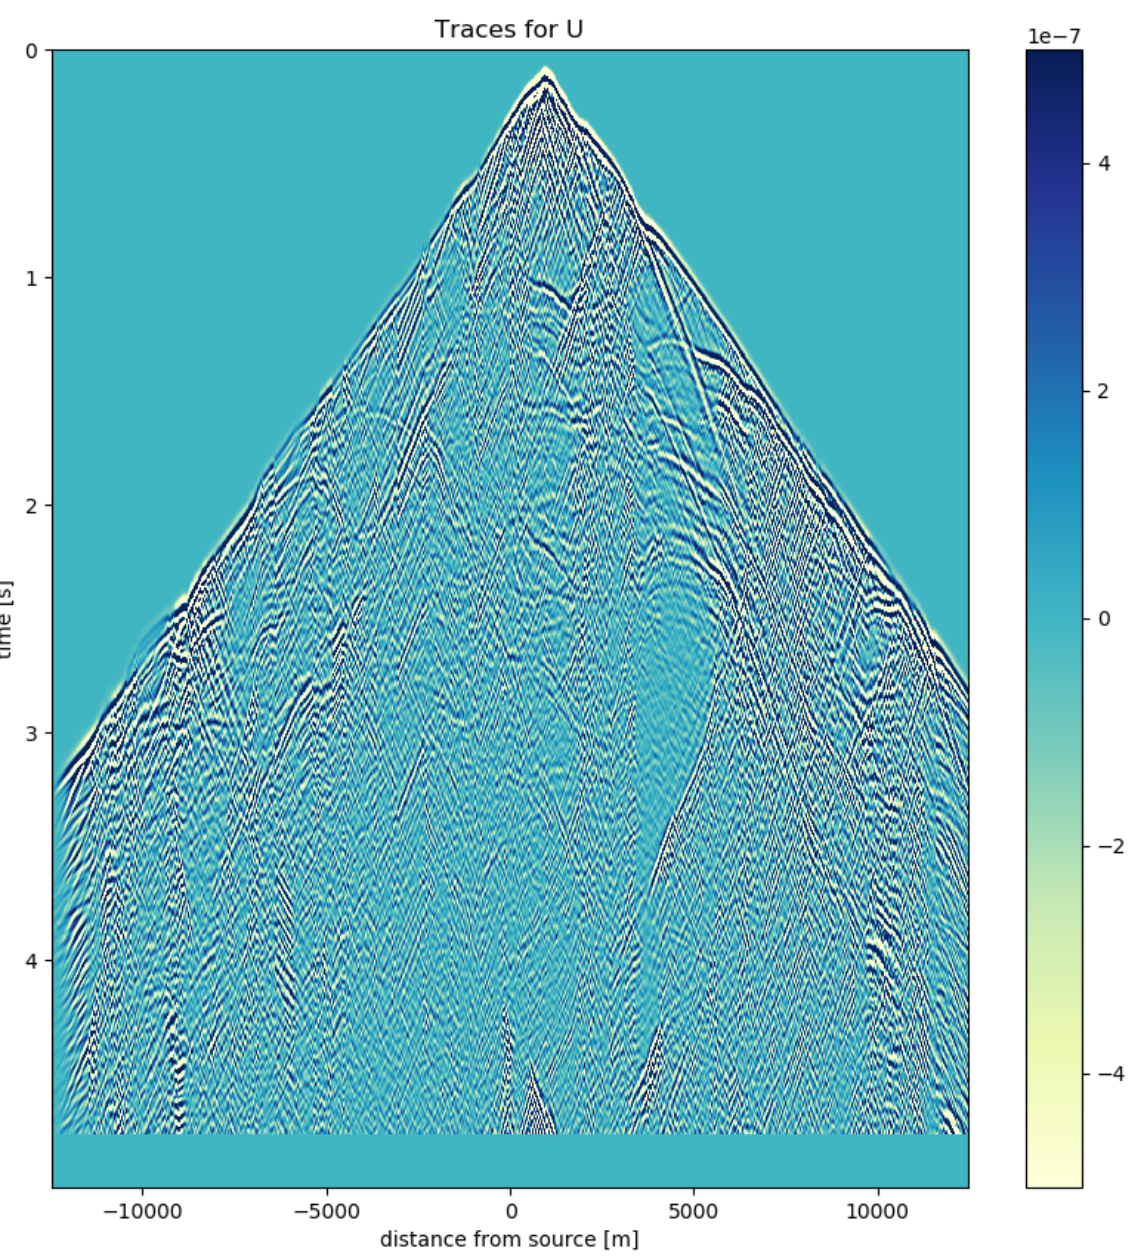
\includegraphics[width=0.55\linewidth]{fig/candian_shots_u_test}
%}
%\subfloat[][]{
%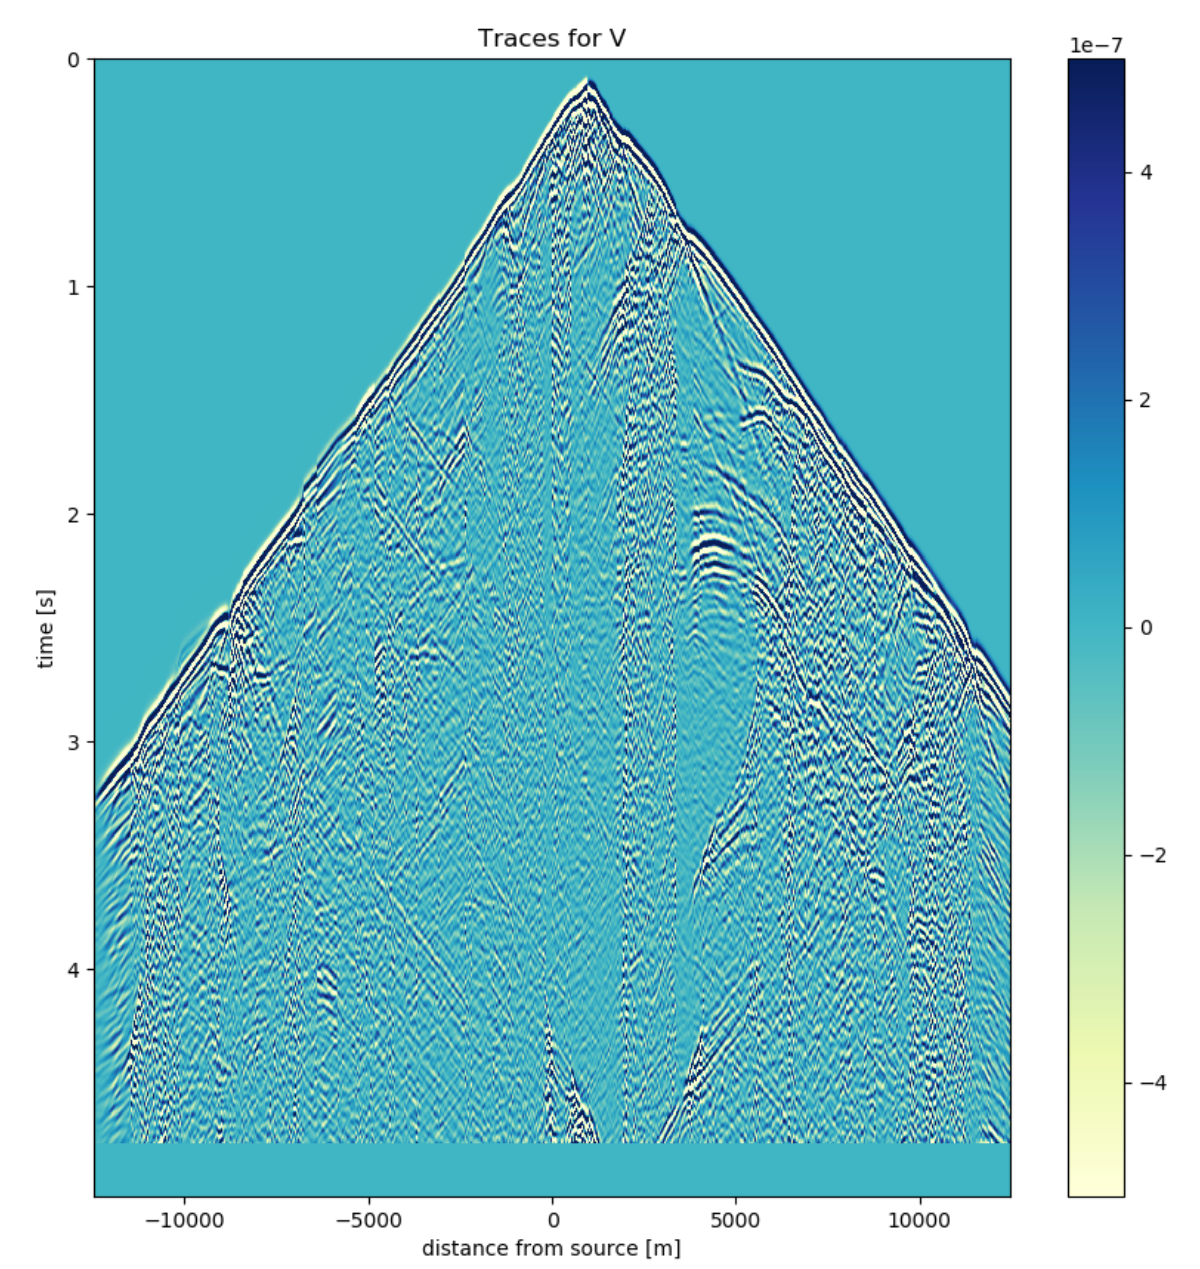
\includegraphics[width=0.56\linewidth]{fig/canadian_shots_v_test}
%}
%\caption{Elastic wave propagation in homogeneous media. Top 4 images show the simulation with reflecting boundary conditions and the bottom four with CPML active, giving a clear decrease in reflection amplitude. $V_p=2500$m/s, $V_s=430$m/s, $\rho=1750$m/s, $f_{source}=10$Hz, $n_x=n_z=220$, $d_x=d_z=10$m, $dt=0.3$ms}
%\label{fig:shots_canadian}
%\end{figure}

%\begin{figure}
%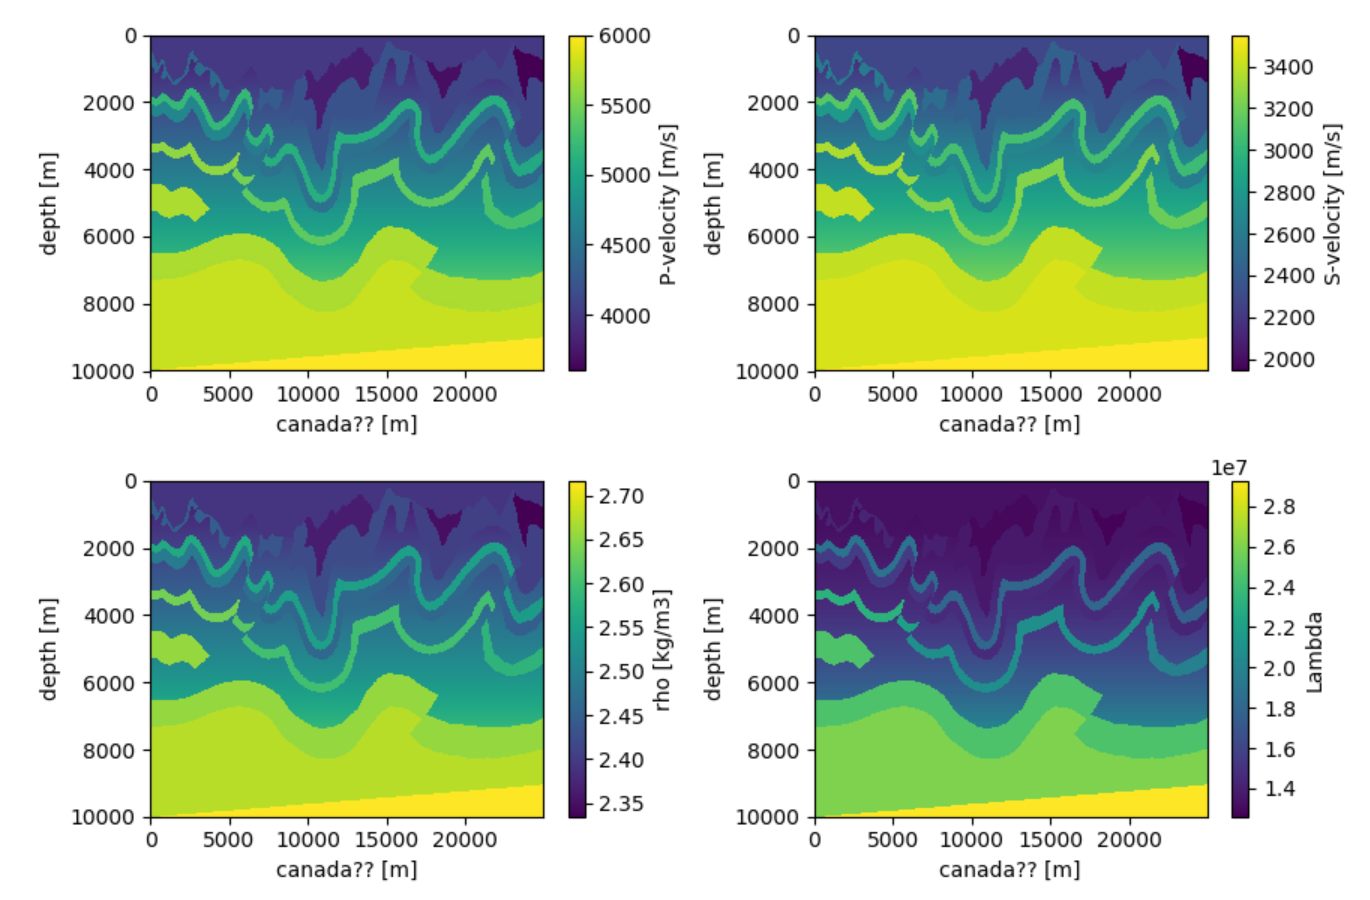
\includegraphics[width=1\textwidth]{fig/canadian_model_test.PNG}
%\end{figure}

\section{Implementation Full Waveform Inversion}

\subsection{Adjoint back-propagation}
To avoid approximating $\pder[\chi]{dm}$ numerically by evaluating the forward model at least  $2 \times N_x \times N_z$ times we use the adjoint state method as described in~\cref{sec:discretized_math}. The discrete version of our derived set of continuous equations given in~\cref{eq:elastic_adjoint} is for a central 2nd order in time and arbitrary order in space by
\begin{equation}\label{eq:discretized_elastic_adjoint_written_out}
    \begin{aligned}
    \overline{U}^{n-\frac{1}{2}}_{i,j} &= \overline{U}^{n+\frac{1}{2}}_{i,j} - \frac{\Delta t}{\rho_{i,j}} \left(D_x\left[\left(\lambda_{i,j} + 2\mu_{i,j}\right)\overline{X}_{i,j}^n\right] + D_x\left[\lambda_{i,j} \overline{Z}^n_{i,j}\right] + D_z\left[\mu_{i,j}\overline{T}_{i,j}^n\right] \right) \\
    \overline{Z}^{n-\frac{1}{2}}_{i+\frac{1}{2},j+\frac{1}{2}} &= \overline{Z}^{n+\frac{1}{2}}_{i+\frac{1}{2}, j+\frac{1}{2}} - \frac{\Delta t}{\rho_{i+\frac{1}{2},j+\frac{1}{2}}} \left(D_z\left[\lambda_{i+\frac{1}{2},j+\frac{1}{2}}\overline{X}_{i+\frac{1}{2},j+\frac{1}{2}}^n\right] + D_z\left[\left(\lambda_{i+\frac{1}{2},j+\frac{1}{2}}+2\mu_{i+\frac{1}{2},j+\frac{1}{2}}\right) \overline{Z}^n_{i+\frac{1}{2},j+\frac{1}{2}}\right]\right. \\
    &\left.+ D_x\left[\mu_{i+\frac{1}{2},j+\frac{1}{2}}\overline{T}_{i+\frac{1}{2},j+\frac{1}{2}}^n\right] \right) \\
    \overline{X}_{i+\frac{1}{2},j}^{n} &= \overline{X}_{i+\frac{1}{2},j}^{n+1} - \Delta t D_x\left[\overline{U}^{n+\frac{1}{2}}_{i+\frac{1}{2},j}\right] \\
    \overline{Z}_{i+\frac{1}{2},j}^{n} &= \overline{Z}_{i+\frac{1}{2},j}^{n+1} - \Delta t D_z\left[\overline{V}^{n+\frac{1}{2}}_{i+\frac{1}{2},j}\right] \\
    \overline{T}_{i,j+\frac{1}{2}}^{n} &= \overline{T}_{i,j+\frac{1}{2}}^{n+1} - \Delta t \left(D_z\left[\overline{U}^{n+\frac{1}{2}}_{i,j + \frac{1}{2}}\right] + D_x\left[\overline{V}^{n+\frac{1}{2}}_{i,j + \frac{1}{2}}\right]\right) \\
\end{aligned}
\end{equation}
where the adjoint versions of the corresponding forward fields are denoted with a line above the letter. The discrete differential operators in direction $s\in\{x,z\}$ are denoted by $D_s\left[\circ\right]$. Note that it is important that the parameters are multiplied with the fields \emph{before} the differentiation is applied. For example with a 2nd order central finite difference $D_z\left[\lambda_{i+\frac{1}{2},j+\frac{1}{2}}\overline{X}_{i+\frac{1}{2},j+\frac{1}{2}}^n\right] = \frac{1}{\Delta_z}\left(\lambda_{i+\frac{1}{2},j+1}\overline{X}_{i+\frac{1}{2},j+1}^n - \lambda_{i+\frac{1}{2},j}\overline{X}_{i+\frac{1}{2},j}^n\right)$. Also note the swapping and sign difference of $n, n+1$ with respect to the forward equations since we are backpropagating from $t=T_{final}$ to $0$. 

A CPML layer was also implemented for the adjoint equations. The method to derive the equations inside the CPML layer was the same as for the forward equations and simply consisted of adding memory variables to each derivative present in~\cref{eq:discretized_elastic_adjoint_written_out}. The parameters for CPML used where the same as in the forward model and this thus resulted in a total of 8 extra 2D fields (memory variables) being stored in the adjoint CPML area. 

\begin{algorithm}
\caption{Backward adjoint modeling and gradient calculation}\label{alg:adjoint_prop}
\begin{algorithmic}[1]
\Function{Propagate adjoint and calculate gradients}{$U,V$}
\Comment{Beginning of adjoint loop}
\State $\gamma_{\rho} = 0, \gamma_{\mu} = 0, \gamma_{\lambda} = 0$ \Comment{Initialize gradients to 0}
\State $\overline{U} \gets \overline U - \left(d^{mod}_U\left(N_t-1\right) - d^{meas}_U\left(N_t-1\right)\right) $ \Comment{~\cref{eq:adjoint_source}}
\State $\overline{Z} \gets \overline Z - \left(d^{mod}_Z\left(N_t-1\right) - d^{meas}_Z\left(N_t-1\right)\right) $
    \For{$it = 1$ to $it < N_t$}
    \State $\overline X, \overline Z, \overline T \gets $ \Call{Propagate Adjoint Stress}{$\overline U, \overline V$} \Comment{Step \cref{eq:discretized_elastic_adjoint_written_out}}
    \State $\overline U, \overline V \gets $ \Call{Propagate Adjoint Velocity}{$\overline X, \overline Z, \overline T$} 
    \State  \Comment{add residuals from~\cref{eq:adjoint_source} as source to the adjoint fields of $V_x$ and $V_z$}
    \State $\overline{U} \gets \overline U - \left(d^{mod}_U\left(N_t-1-it\right) - d^{meas}_U\left(N_t-1-it\right)\right) $ \Comment{~\cref{eq:adjoint_source}}
    \State $\overline{Z} \gets \overline Z - \left(d^{mod}_Z\left(N_t-1-it\right) - d^{meas}_Z\left(N_t-1-it\right)\right) $
    \State $it \gets it + 1$
    \State $\gamma_{\rho}, \gamma_{\mu}, \gamma_{\lambda} \gets $\Call{step gradients}{$it,U,V,\overline{U}, \overline{V}, \overline{X}, \overline{Z}, \overline{T}$} \Comment{Add steps of the sum of eq~\cref{eq:discrete_gradient_rho_written_out,eq:discrete_gradient_mu_written_out,eq:discrete_gradient_lambda_written_out} to the gradients}
    \EndFor
\EndFunction
\end{algorithmic}
\end{algorithm}

\subsection{Gradient calculation}
The gradient is calculated following~\cref{eq:gradient_discretised_linear} using the same notation as in~\cref{eq:discretized_elastic_adjoint_written_out,eq:elastic_discretized_written_out}. A 2nd order central difference in space and time was used. For $\rho$ we get 
\begin{equation}\label{eq:discrete_gradient_rho_written_out}
\pder[\chi]{\rho} \approx \sum_{n=0}^{N_t-1}\sum_{i=0}^{N_x-1}\sum_{j=0}^{N_z-1} \frac{1}{2}\left[\overline{U}^{n+\frac{1}{2}}_{i,j}\left(U_{i,j}^{n+1\frac{1}{2}} - U^{n-\frac{1}{2}}_{i,j}\right) + \overline{V}^{n+\frac{1}{2}}_{i+\frac{1}{2},j+\frac{1}{2}}\left(V_{i+\frac{1}{2},j+\frac{1}{2}}^{n+1\frac{1}{2}} - V^{n-\frac{1}{2}}_{i+\frac{1}{2},j+\frac{1}{2}}\right)\right]\Delta x \Delta z
\end{equation}
where we used a 2nd order in time central difference of $2\Delta t$ to make the fields coincide with our choice of staggered grid. For $\lambda$ we get
\begin{equation}\label{eq:discrete_gradient_lambda_written_out}
\begin{aligned}
\pder[\chi]{\lambda} &\approx \sum_{n=0}^{N_t-1}\sum_{i=0}^{N_x-1}\sum_{j=0}^{N_z-1} \left(\overline{X}^n_{i+\frac{1}{2}, j} + \overline{Z}^n_{i+\frac{1}{2}, j}\right) \left[\frac{1}{2\Delta x}\left(\left(U^{n-\frac{1}{2}}_{i+1,j} + U^{n+\frac{1}{2}}_{i+1,j}\right) - \left(U^{n-\frac{1}{2}}_{i,j} + U^{n+\frac{1}{2}}_{i,j}\right)\right) \right. \\
&+\left. \left(\left(V^{n-\frac{1}{2}}_{i+\frac{1}{2},j+\frac{1}{2}} + V^{n+\frac{1}{2}}_{i+\frac{1}{2},j+\frac{1}{2}}\right) - \left(V^{n-\frac{1}{2}}_{i+\frac{1}{2},j-\frac{1}{2}} + V^{n+\frac{1}{2}}_{i+\frac{1}{2},j-\frac{1}{2}}\right)\right)   \right]\Delta x \Delta z \Delta t
\end{aligned}
\end{equation}
and for $\mu$ we get
\begin{equation}\label{eq:discrete_gradient_mu_written_out}
\begin{aligned}
\pder[\chi]{\mu} \approx \sum_{n=0}^{N_t-1}\sum_{i=0}^{N_x-1}\sum_{j=0}^{N_z-1}&\left\{ -\frac{1}{\Delta x}\overline{X}^n_{i+\frac{1}{2}, j} \left[\left(U^{n-\frac{1}{2}}_{i+1,j} + U^{n+\frac{1}{2}}_{i+1,j}\right) - \left(U^{n-\frac{1}{2}}_{i,j} + U^{n+\frac{1}{2}}_{i,j}\right)\right]\right. \\
&\left.-  \frac{1}{\Delta z}\overline{Z}^n_{i+\frac{1}{2}, j}\left[\left(V^{n-\frac{1}{2}}_{i+\frac{1}{2},j+\frac{1}{2}} + V^{n+\frac{1}{2}}_{i+\frac{1}{2},j+\frac{1}{2}}\right) - \left(V^{n-\frac{1}{2}}_{i+\frac{1}{2},j-\frac{1}{2}} + V^{n+\frac{1}{2}}_{i+\frac{1}{2},j-\frac{1}{2}}\right)\right]  \right.\\
&\left.-\frac{1}{2\Delta z}\overline{T}^n_{i,j+\frac{1}{2}}\left[\left(U^{n+\frac{1}{2}}_{i,j+1} + U^{n-\frac{1}{2}}_{i,j+1}\right) - \left(U^{n+\frac{1}{2}}_{i,j} + U^{n-\frac{1}{2}}_{i,j}\right)  \right]\right.\\
& \left.-\frac{1}{2\Delta x}\overline{T}^n_{i,j+\frac{1}{2}}\left[\left(V^{n+\frac{1}{2}}_{i+\frac{1}{2},j+\frac{1}{2}} + V^{n-\frac{1}{2}}_{i+\frac{1}{2},j+\frac{1}{2}}\right) - \left(V^{n+\frac{1}{2}}_{i-\frac{1}{2},j+\frac{1}{2}} + V^{n-\frac{1}{2}}_{i-\frac{1}{2},j+\frac{1}{2}}\right)  \right]\right\}\Delta x \Delta z \Delta t
\end{aligned}
\end{equation}
where again we interpolated in time by averaging a field $K$ at $K^n_{i,j} \approx \frac{1}{2}\left(K^{n+\frac{1}{2}}_{i,j} + K^{n-\frac{1}{2}}_{i,j}\right)$.
\subsection{Model updating using L-BFGS gradient descent}
With the gradients in hand, the most simple way to update the models in the gradient direction would just be at each iteration descend in the negative gradient direction. 
\begin{equation}\label{eq:simplest_gradient_descend}
\left\{
\begin{aligned}
\vec{\rho}_k &= \vec{\rho}_{k-1} - \alpha^{\rho}_k\gamma_\rho \\
\vec{\lambda}_k &= \vec{\lambda}_{k-1} - \alpha^{\lambda}_k\gamma_\lambda \\
\vec{\mu}_k &= \vec{\mu}_{k-1} - \alpha^{\mu}_k\gamma_\mu
\end{aligned}
\right.
\end{equation}
where the index $k$ denotes the iteration number, $\alpha^{\rho}_k, \alpha^{\lambda}_k, \alpha^{\mu}_k $ are step dependent positive stepsizes and the gradients $\vec{\gamma_m}=\pder[\chi]{\vec{m}}\ \forall\  \vec{m} \in \left\{\vec{\rho},\vec{\mu},\vec{\lambda}\right\}$ . In practice, with simple gradient descend, these are constant during the iterations and are determined by hand by monitoring the cost function until it decreases sufficiently each iteration.

Now \emph{Newton's method} for finding roots of function is often used in optimization due to it's incorporation of curvature information through the second derivative(or Hessian Matrix $H$ in multi-dimensional problems). Newton's method improves on~\cref{eq:simplest_gradient_descend} by adding this Hessian information in the gradient descend according to
\begin{equation}\label{eq:newtons_method_grad_descend}
\begin{aligned}
\vec{\rho}_k &= \vec{\rho}_{k-1} - \alpha^{\rho}_k H_{\rho_k}^{-1} \gamma_\rho \\
\vec{\lambda}_k &= \vec{\lambda}_{k-1} - \alpha^{\lambda}_k H_{\lambda_k}^{-1} \gamma_\lambda \\
\vec{\mu}_k &= \vec{\mu}_{k-1} - \alpha^{\mu}_k H_{\mu_k}^{-1} \gamma_\mu
\end{aligned}
\end{equation}
The inverse Hessian matrix $H^{-1}$ is computationally expensive to calculate, which is why \emph{quasi-Newton methods} were introduced, approximating the Hessian. One particular widely used version is the Broyden–Fletcher–Goldfarb–Shannon (BFGS) algorithm and it's limited memory variant L-BFGS~\cite{Liu1989}. This tries to approximate the product of the inverse Hessian and gradient by using information of the previous gradient descend steps( and thus requiring one to save the last $L$ previous models and gradients costing extra memory). In this work we used a pre-written standalone module in C~\cite{Alberto2018} which we fed the calculated gradients and models each iteration and which returned the product $H^{-1}\pder[\chi]{\vec{m}}$ for each parameter separately.

\subsection{Implementation in C}
The FWI inversion for the elastic wave equation was implemented in C in combination with Madagascar\cite{m8r} for reproducible workflow, Jupyter-notebook\cite{Kluyver2016} for data analysis and plotting and is available on request.\footnote{contact: Jaapwesdorp@gmail.com}. 

\subsubsection{Memory considerations}
The forward modeling of the elastic wave equation in principle only requires one to store 14 $N_x \times N_z$ fields (3 models, 5 real fields and 6 CPML memory variables, which could be optimized to be only the size of the CPML layer at the cost of code clarity). And at each timestep the memory can be overwritten. For the adjoint back-propagation we have the same and thus need to store 13 more fields(5 + 8 CPML). The problem with gradients is that we need to calculate the product of the adjoint and forward fields at all timesteps. We thus need to store the time-slices of at least one of the two. We therefore stored $U$ and $V$ as 3D fields of size $N_x \times N_z \times N_t$ and calculated the gradient during the adjoint propagation loop (approximating $D_t U, D_t V, D_xU, D_xV, D_zU$ and $D_z V$ during the adjoint loop instead of saving these 6 fields in the forward propagation). This provided the best trade-off between memory and computational cost, since memory was a real issue on the 16Gb RAM PC. The full algorithm is shown in~\cref{alg:full_fwi}


\begin{algorithm}
\caption{FWI sequence}\label{alg:full_fwi}
\begin{algorithmic}[1]
\State $d^{meas}_U, d^{meas}_V \gets $\Call{read measured shots}{ } \Comment{Read measured shot data at all receiver positions}
\State $\rho, \mu, \lambda \gets $ \Call{read initial models}{ }
\State 
\For{$k=0$ to $k < N_{fwi-iterations}$}
    \For{\textbf{each source} $f_q$} \Comment{Loop over source positions(in parallel)}
        \State $U, V \gets $ \Call{propagate forward}{$\rho, \mu, \lambda$} \Comment{Save the 3D forward velocities for gradients}
        \State $d^{mod}_U, d^{mod}_V \gets $\Call{save modeled shots}{$U,V$} \Comment{Save shots at all receiver positions}
   
        \State $\gamma_{\rho}, \gamma_{\mu}, \gamma_{\lambda} \gets $ \Call{propagate adjoint and calculate gradients}{$U,V, \rho, \mu, \lambda$} \Comment{\cref{alg:adjoint_prop}}
    \EndFor
    \If{$k < n_{\text{gradient descend}}$} \Comment{Perform initial gradient descend steps}
        \State $\rho \gets \rho - \alpha^{\rho}_k \gamma_{\rho}$ \Comment{Stepsize $\alpha$ determined by hand}
        \State $\mu \gets \mu - \alpha^{\mu}_k \gamma_{\mu}$
        \State $\lambda \gets \lambda - \alpha^{\lambda}_k \gamma_{\lambda}$
    \Else  \Comment{Perform L-BFGS steps}
        \State $c_k \gets 0$ \Comment{Initialize cost function}
        \State $\alpha^{\rho}_k, \alpha^{\mu}_k, \alpha^{\mu}_k \gets 1$ \Comment{Set initial L-BFGS stepsize to 1}
        \State $\tilde{H}_{\rho}^{-1}\gamma_{\rho}, \tilde{H}_{\mu}^{-1}\gamma_{\mu}, \tilde{H}_{\lambda}^{-1}\gamma_{\lambda} \gets$ \Call{approximate hessians via L-BFGS}{$k,\rho, \mu, \lambda, \gamma_\rho, \gamma_\mu, \gamma_\lambda$}
        \State $\rho \gets \rho - \alpha^{\rho}_k \tilde{H}_{\rho}^{-1}\gamma_{\rho}$ 
        \State $\mu \gets \mu - \alpha^{\mu}_k \tilde{H}_{\mu}^{-1}\gamma_{\mu}$
        \State $\lambda \gets \lambda - \alpha^{\lambda}_k \tilde{H}_{\lambda}^{-1}\gamma_{\lambda}$
        \For{\textbf{each source} $f_q$} 
        \State $U, V \gets $ \Call{propagate forward}{$\rho, \mu, \lambda$}  \Comment{Redo the forward modeling}
        \State $d^{mod}_U, d^{mod}_V \gets $\Call{save modeled shots}{$U,V$} 
        \State $c_k \gets $ \Call{calculate cost function}{$d^{meas}_U, d^{meas}_V, d^{mod}_U, d^{mod}_V$} \Comment{\cref{eq:cost_function_standard}}
        \EndFor
        \While{$c_k > c_{k-1}$} \Comment{Enter L-BFGS attempt loop if cost is not decreasing}
            \State $\alpha^{\rho}_k \gets \frac{1}{2}\alpha^{\rho}_k,\  \alpha^{\mu}_k\gets \frac{1}{2}\alpha^{\mu}_k,\ \alpha^{\lambda}_k\gets \frac{1}{2}\alpha^{\lambda}_k$
            \State $\rho \gets \rho + \alpha^{\rho}_k \tilde{H}_{\rho}^{-1}\gamma_{\rho}$ \Comment{Add back half the step taken}
            \State $\mu \gets \mu + \alpha^{\mu}_k \tilde{H}_{\mu}^{-1}\gamma_{\mu}$
            \State $\lambda \gets \lambda + \alpha^{\lambda}_k \tilde{H}_{\lambda}^{-1}\gamma_{\lambda}$
            \For{\textbf{each source} $f_q$} 
            \State $U, V \gets $ \Call{propagate forward}{$\rho, \mu, \lambda$} \Comment{Redo the forward modeling}
            \State $d^{mod}_U, d^{mod}_V \gets $\Call{save modeled shots}{$U,V$} 
            \State $c_k \gets $ \Call{calculate cost function}{$d^{meas}_U, d^{meas}_V, d^{mod}_U, d^{mod}_V$} 
            \EndFor
        \EndWhile
    \EndIf

\EndFor
\end{algorithmic}
\end{algorithm}
\clearpage
\section{FWI results}
FWI was tested on a synthetic model (~\cref{fig:cps_model}) with both larger features (the CPS letters) and smaller (research group). The grid size was always $N_x = 113$ by $N_z=214$ points. The grid-spacing was taken to be $\Delta_x = \Delta_z = 10$m and Brocher's relations~\cref{eq:brochers_rho,eq:brochers_vs} were used to calculate $v_s$ and $\rho$ from $v_p$. The central source frequency was $3$Hz (resulting in 54 Points per wavelength (PPW) for P-waves and 14 for S-waves) and the inversion was carried out for 7 sources in parallel denoted by the blue dots in~\cref{fig:cps_model} and receivers at every 10m denoted by the red line.
\begin{figure}[!h]\label{fig:cps_model}
\hspace*{-0.4in}
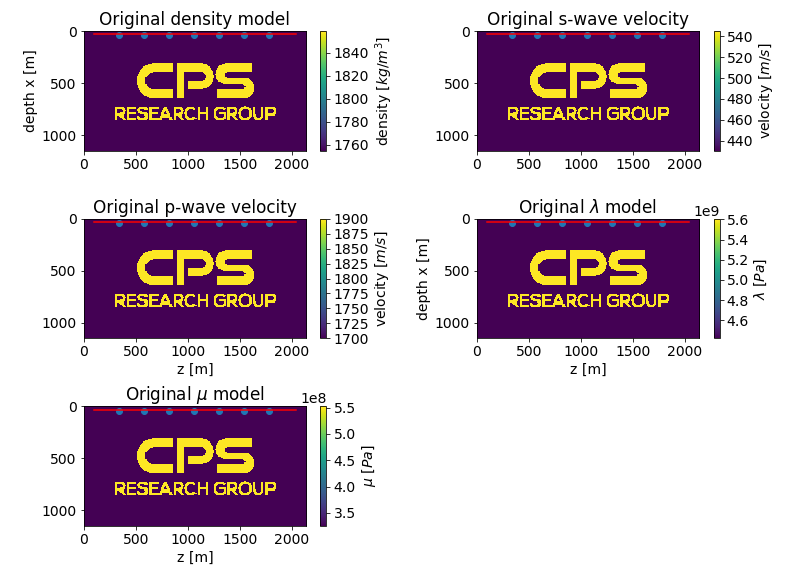
\includegraphics[width=1.15\textwidth]{fig/cps_models2}
\caption{Synthetic models used for testing FWI}
\end{figure}

For the FWI we took 2 standard gradient descend steps before applying L-BFGS. The initial stepsize $\alpha$ was determined by hand for each parameter separately by looking at the first step and taking the value where the cost was sufficiently decreasing. As can be seen later, the range in which this parameter can be chosen for the L-BFGS to be effective spans several orders of magnitude. 

\begin{figure}[!h]\label{fig:cps_fwi_empty_start_single_params}
\hspace*{-0.6in}
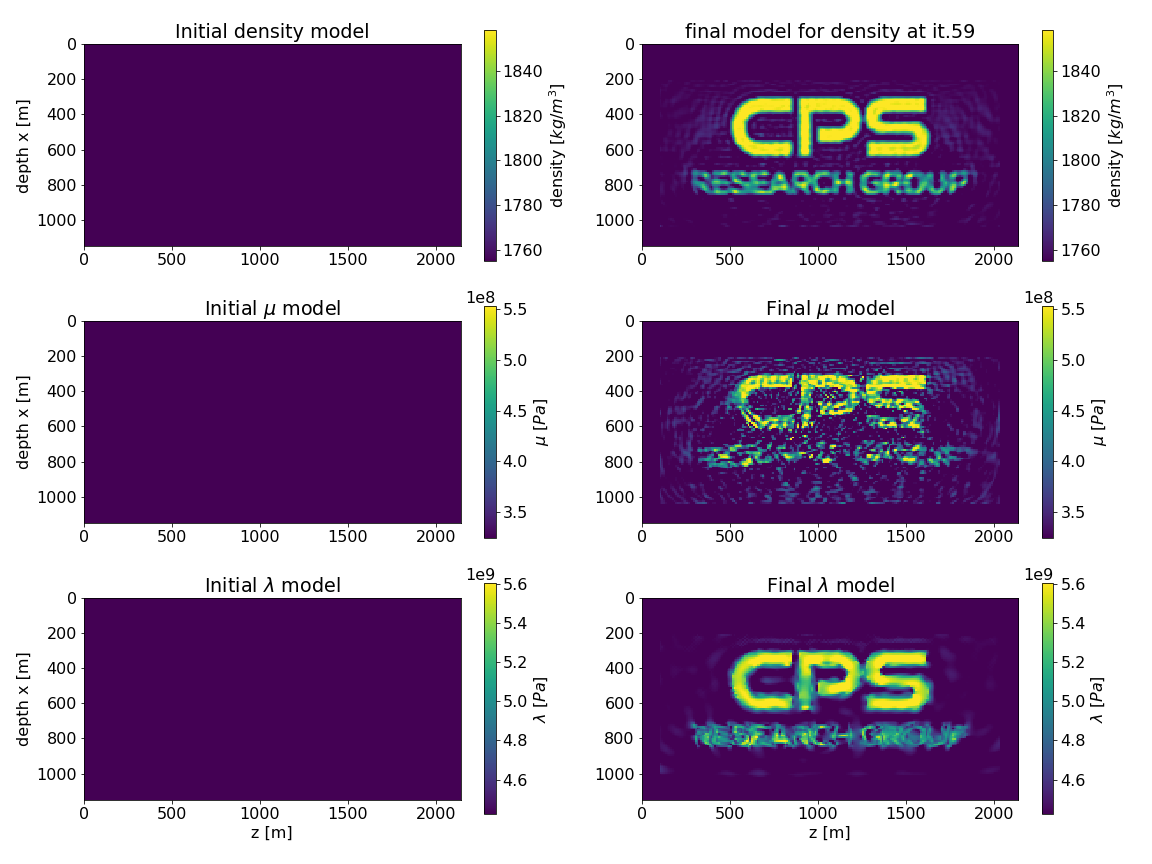
\includegraphics[width=1.20\textwidth]{fig/fwi_cps_single_param6s.png}
\hspace*{-0.6in}
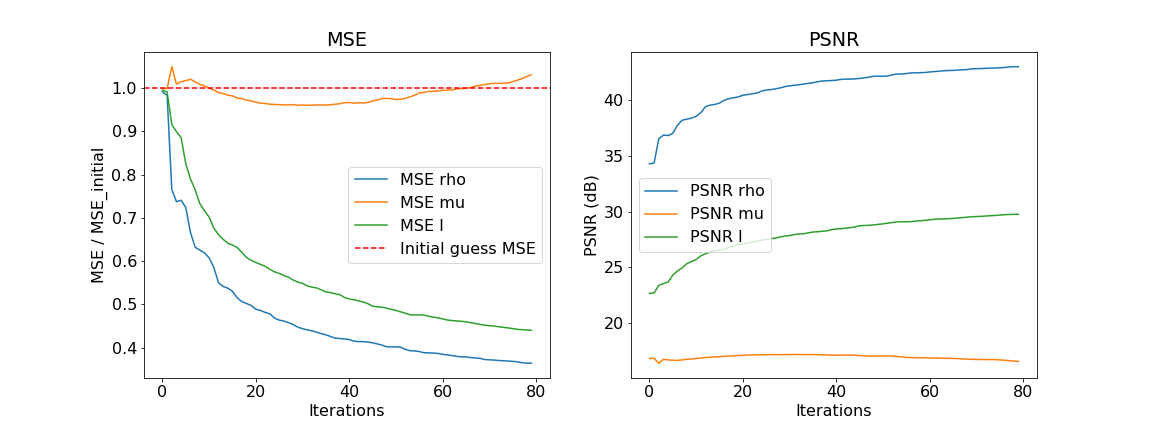
\includegraphics[width=1.20\textwidth]{fig/fwi_cps_single_param6s_error.png}
\caption{One by one sequential single parameter inversion with an empty homogeneous starting model with the other two parameters held fixed on the original and the original taken as~\cref{fig:cps_model}}
\end{figure}


\begin{figure}[!h]\label{fig:cps_fwi_empty_start}
\hspace*{-0.6in}
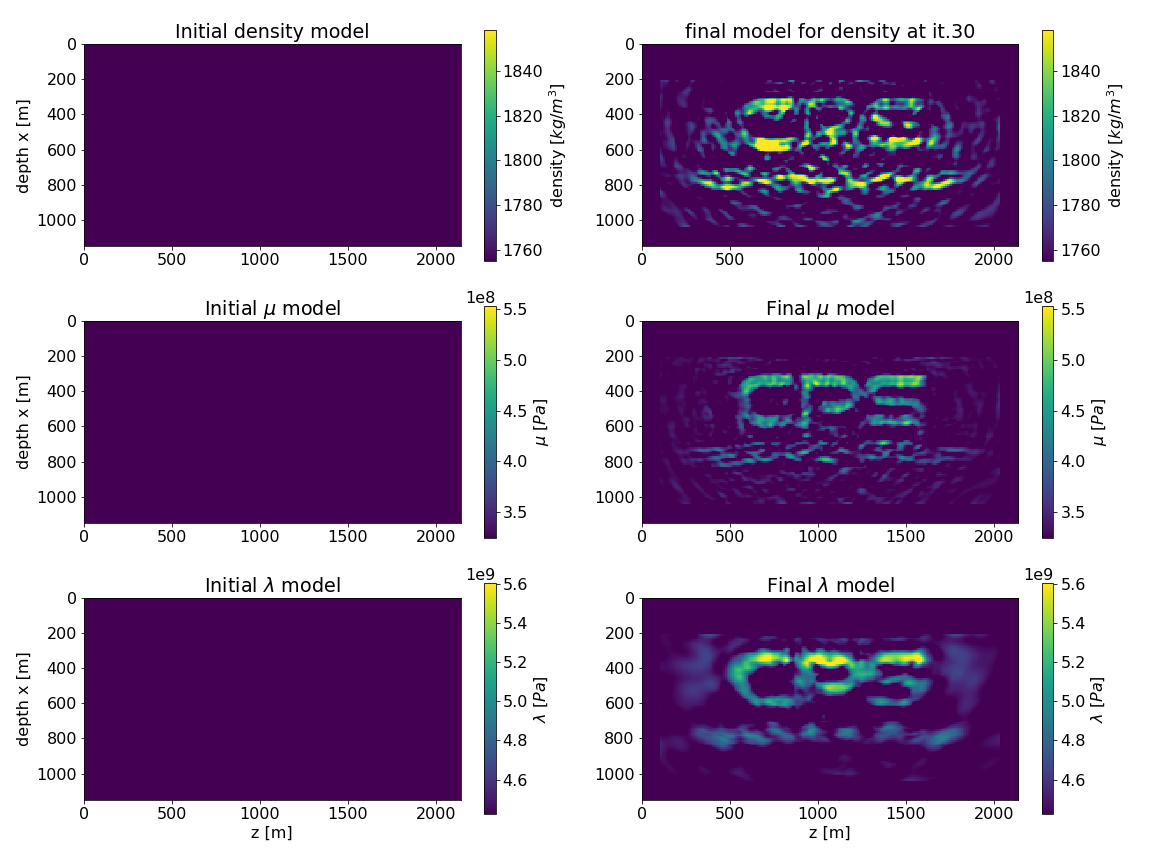
\includegraphics[width=1.20\textwidth]{fig/cps_fwi_three_params}
\hspace*{-0.6in}
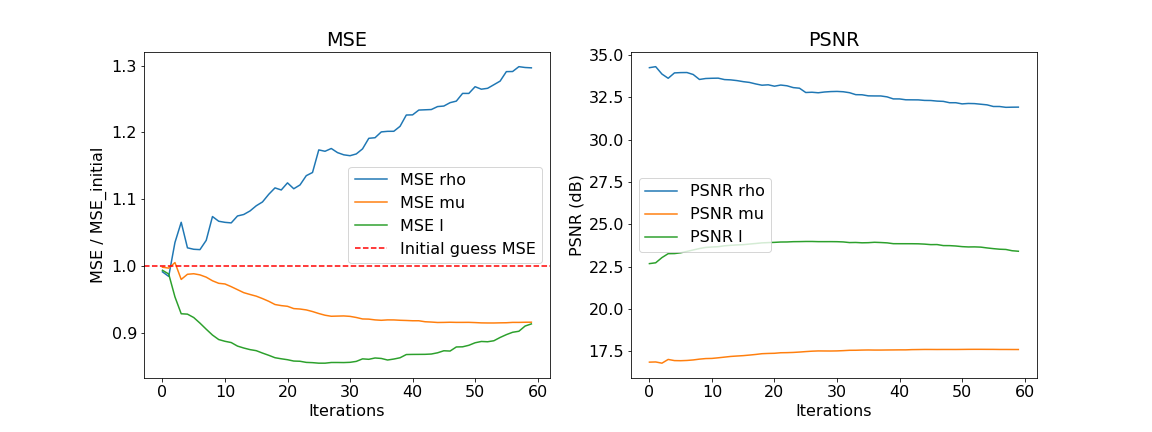
\includegraphics[width=1.20\textwidth]{fig/cps_fwi_three_params_MSE}
\caption{Three parameter inversion result with a homogeneous starting model and the original taken as~\cref{fig:cps_model}}
\end{figure}
\begin{figure}[!h]\label{fig:cps_fwi_smooth_start}
\hspace*{-0.6in}
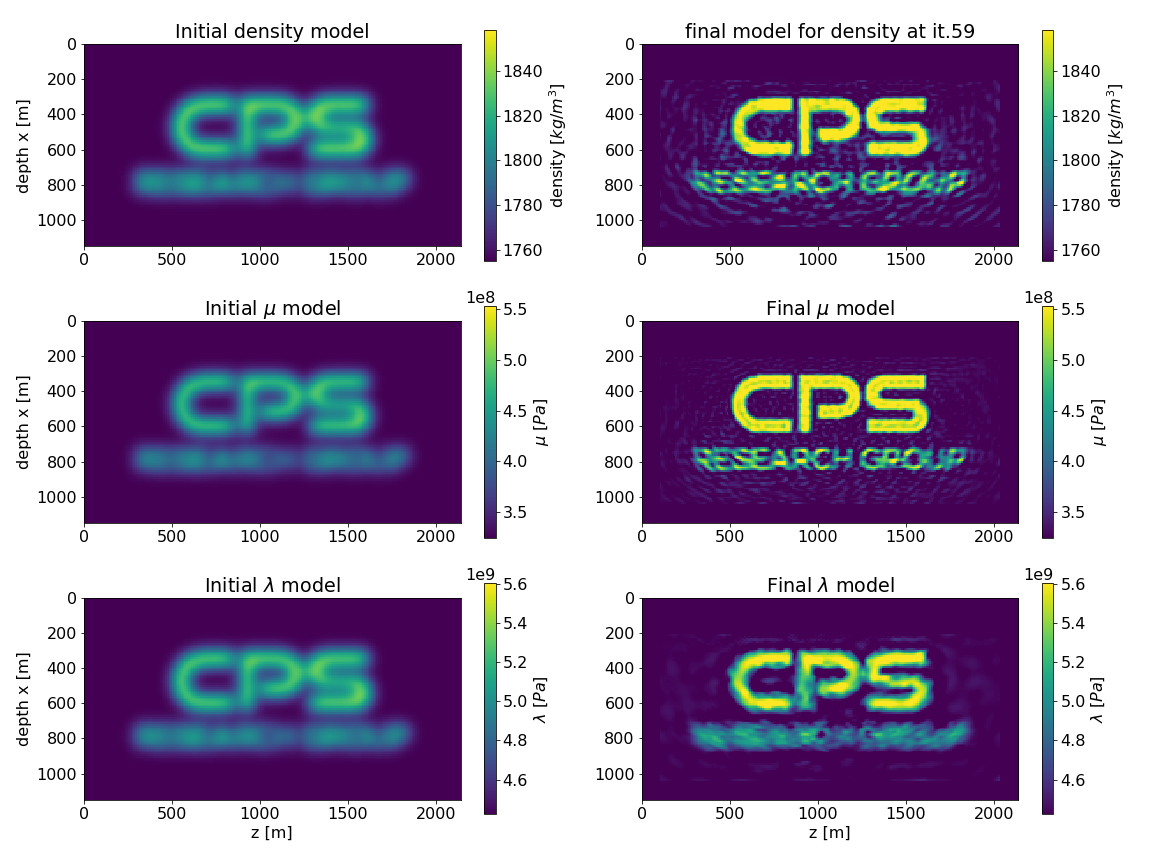
\includegraphics[width=1.20\textwidth]{fig/cps_fwi_three_params_smooth}
\hspace*{-0.6in}
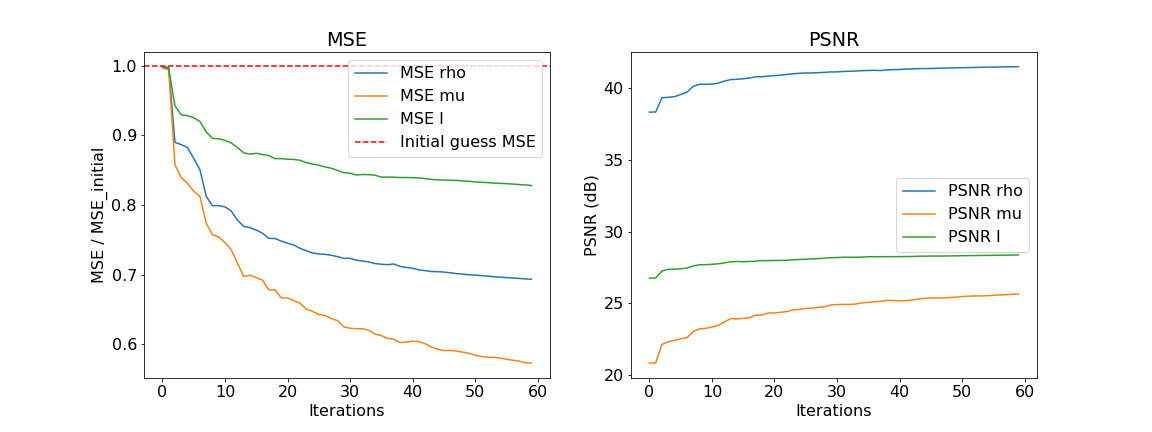
\includegraphics[width=1.20\textwidth]{fig/cps_fwi_three_params_smooth_MSE}
\caption{Three parameter inversion result with a smooth starting model and the original taken as~\cref{fig:cps_model}}
\end{figure}
\begin{figure}[!h]\label{fig:cps_alpha_comparison}
\hspace*{-0.4in}
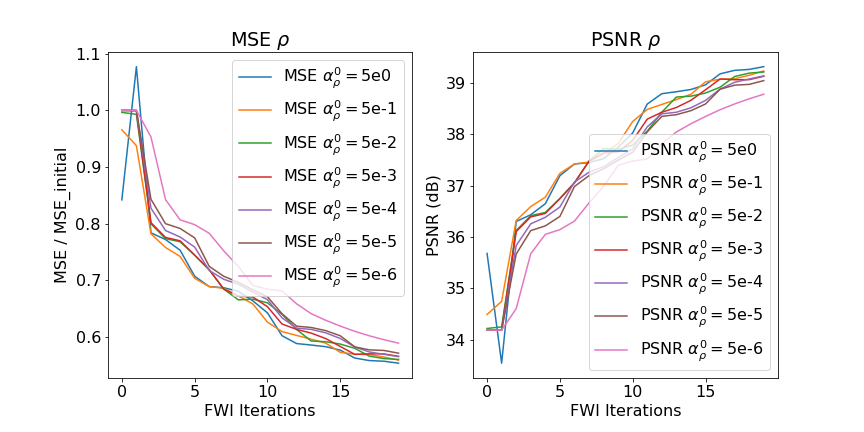
\includegraphics[width=1.15\textwidth]{fig/alpha_comparison}
\caption{Comparison of final errors and PSNR for different initial stepsizes.}
\end{figure}

\begin{figure}[!h]\label{fig:cps_n_receiver_comparison}
\hspace*{-0.4in}
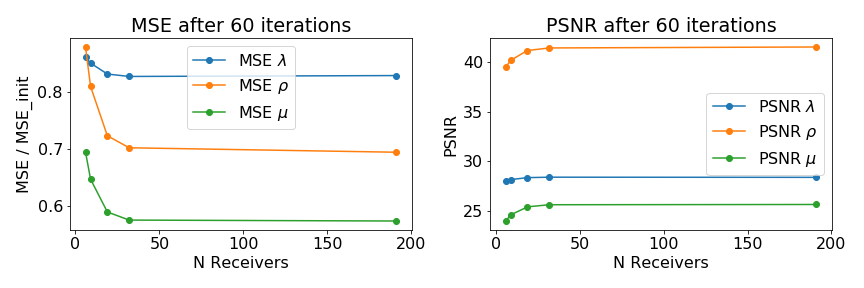
\includegraphics[width=1.15\textwidth]{fig/fwi_vs_n_receivers.png}
\caption{Final reconstruction quality with varying amount of receivers. The reconstruction was performed with the smooth starting model from~\cref{fig:cps_fwi_smooth_start} for varying $N_R \in \left\{191,32,19,9,6\right\}$}
\end{figure}

\begin{figure}[!h]\label{fig:cps_gridsize_comparison}
\hspace*{-0.4in}
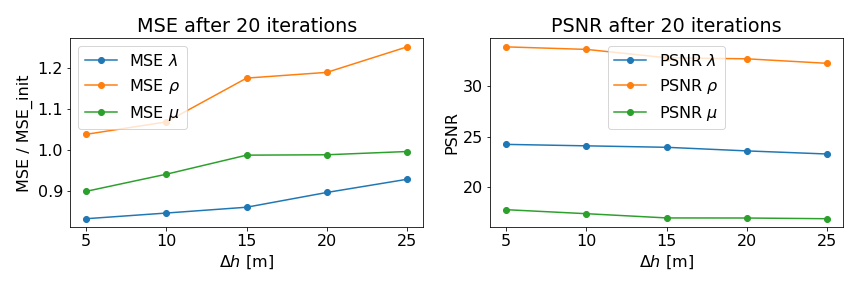
\includegraphics[width=1.15\textwidth]{fig/fwi_vs_gridsize.png}
\caption{Final reconstruction quality of CPS model with homogeneous starting model with varying gridsize $\Delta h = \Delta x = \Delta z$ the propagation time was increased with gridsize linearly to make sure the wave always propagated the same distance. As gridsize increases, the amount of PPW decreases and therefore the reconstruction quality. Because the amount of points were fixed due to memory limitations, the physical size of the letters increased with $\Delta h$ which in prinicple should increase the reconstruction quality.}
\end{figure}

\clearpage
%--------------------------------------------------------------------------------------------------------------------

\section{Conclusion}

%--------------------------------------------------------------------------------------------------------------------



%------------------------------------------------
%\phantomsection
%\section*{Acknowledgments} % The \section*{} command stops section numbering

%\addcontentsline{toc}{section}{Acknowledgments} % Adds this section to the table of contents

%So long and thanks for all the fish

\appendix
\section*{Appendices}
\addcontentsline{toc}{section}{Appendices}
\section{Lagrangian based derivation of the gradient via the adjoint state method}\label{sec:general_math}
In this section the adjoint equations and the gradients for a general first or second order PDE system will be derived performing a more generalized version of the approach outlined in \cite{Bradley2012}.
\subsection{General system of equations}
\label{sec:general_system}
We can write the most general minimization problem of a cost function subject any first order or second order (in time) set of partial differential equations(PDE) in the following form
\begin{equation}
\label{eq:general_system}
\begin{aligned}
\underset{m}{\text{min}} &&  \chi\left(s,m\right) = &  \int_0^T f\left(s,m\right) dt & &\\
\text{subject to} & & h\left(\ddot{s}, \dot{s}, s, m, t\right) & =  0 \\
 \text{with B.C} & & g\left((s\left(0\right), m\right) & = 0 \\
 & & k\left((\dot{s}\left(0\right), m\right) & = 0 \\
\end{aligned}
\end{equation}
where $s$ is a discretized vector of the fields and the dots denote derivatives to time, $m$ is the vector of all the discretized model parameters, $t$ denotes time, $h\left(\ddot{s}, \dot{s}, s, m, t\right)  =  0$ is the system of equations, e.g the wave equation in 2D or 3D,$T$ is the final time of integration and $g\left((s\left(0\right), m\right), k\left((\dot{s}\left(0\right), m\right)$ denote initial conditions for the field vector $s$ and its derivative $\dot{s}$. Note that this is similar to \cite{Bradley2012} but with the added explicit dependence of both $\dot s$ and $\ddot s$ giving a more general expression for the adjoint equations and the gradients. 

\subsection{Derivative to model parameters}
 When solving the minimization problem numerically, one often uses a method similar to Newton's gradient descend. This thus requires knowledge of the derivative of the cost function $\chi\left(s,m\right)$ to all of the model parameters $m$. Using the chain rule we obtain:
\begin{equation}\label{eq:derivative_of_chi}
\frac{d\chi}{dm} = \frac{\partial \chi}{\partial s}\frac{\partial s}{\partial m} + \frac{\partial \chi}{\partial m}
\end{equation}
This depends on the Frechet derivatives $\frac{\partial s}{\partial m}$ which require at least $3N$ evaluations of the forward model in order to obtain an estimate, we thus want to avoid the calculation of this term. To facilitate this we define the Lagrangian $\mathcal{L}$ by
\begin{equation}\label{eq:lagrangian}
\begin{aligned}
\mathcal{L} =   \int_0^T \left[f\left(s, m \right) + \lambda^T h\left(\ddot s, \dot s, s, m , t\right)\right] dt 
+ \mu ^T g\left((s\left(0\right), m\right)  + \eta^T k\left((\dot{s}\left(0\right), m\right)
\end{aligned}
\end{equation}
where the auxiliary variables $\lambda, \mu, \eta$ have the same length as the discretized field vector $s$.
Note that due to the initial conditions of~\cref{eq:general_system} we have $\frac{d\chi}{dm} = \frac{d\mathcal{L}}{dm}$, where using the chain rule repetitively 
\begin{equation}\label{eq:lagrangian_derivative_general}
\begin{aligned}
\frac{d\mathcal{L}}{dm} & =  \int_0^T \left[ \pder[f]{s} \pder[s]{m} + \pder[f]{m} \right. \\
& \left. + \lambda^T \left(\pder[h]{\ddot s}\pder[\ddot s]{m} + \pder[h]{\dot s} \pder[\dot s]{m} + \pder[h]{s}\pder[s]{m} + \pder[h]{m}\right) \right]dt  \\
& + \mu^T \left(\pder[g]{s(0)} \pder[s(0)]{m} + \pder[g]{m} \right) \\
& + \eta^T \left(\pder[k]{\dot s(0)} \pder[\dot s(0)]{m} + \pder[k]{m} \right)    
\end{aligned}
\end{equation}
This looks intimidating and not really much simpler, but we are still free to choose the expressions for $\lambda, \mu$ and $\eta$. We will choose this such that we can avoid calculating the computationally difficult derivatives $\pder[s]{m}$. But first we need to do some partial integration to get rid of  $\pder[\dot s]{m}$ and $\pder[\ddot s]{m}$.
With a single partial integration we can write
\begin{equation}\label{eq:lagrangian_partial_first_order}
\begin{aligned}
\int^T_0  \lambda^T \pder[h]{\dot s} \pder[\dot s]{m} = \left[\lambda^T \pder[h]{\dot s} \pder[s]{m}\right]^T_0
 - \int_0^T \pder[s]{m}\left(\dot \lambda^T \pder[h]{\dot s} + \lambda^T \pder{t}\pder[h]{\dot s} \right)
\end{aligned}
\end{equation}
and with a double partial integration we can write
\begin{equation}\label{eq:lagrangian_partial_second_order}
\begin{aligned}
\int^T_0  \lambda^T \pder[h]{\ddot s} \pder[\ddot s]{m} &= \left[\lambda^T \pder[h]{\dot s} \pder[\dot s]{m} - \pder[s]{m}\left(\dot \lambda^T \pder[h]{\ddot s} + \lambda^T \pder{t}\pder[h]{\ddot s}\right)  \right]^T_0 \\
 &+ \int_0^T \pder[s]{m}\left(\ddot \lambda^T \pder[h]{\ddot s} + 2 \dot \lambda^T \pder{t}\pder[h]{\ddot s} + \lambda^T \ppder{t}\pder[h]{\ddot s} \right) dt 
\end{aligned}
\end{equation}
So filling this back into~\cref{eq:lagrangian_derivative_general} and regrouping terms gives
\begin{equation}
\begin{aligned}
\frac{d\mathcal{L}}{dm}& = \int_0^T \left[\pder[s]{m}\left( \pder[f]{s} + \ddot \lambda^T \pder[h]{\ddot s}
 + \dot \lambda^T\left(2\pder{t}\pder[h]{\ddot s}- \pder[h]{\dot s}\right)\right.\right. \\
& \left. \left.  + \lambda^T\left(\pder[h]{s} + \ppder{t}\pder[h]{\ddot s} -\pder{t}\pder[h]{\dot s}\right)\right)
 + \pder[f]{m} + \lambda^T \pder[h]{m}\right]dt \\
 &+\left.\left(\mu^T \pder[g]{s(0)} - \lambda^T\pder[h]{\dot s} + \dot \lambda^T \pder[h]{\ddot s} + \lambda^T\pder{t}\pder[h]{\ddot s}\right)\pder[s]{m}\right|_0 \\
 &+ \left. \left(\eta^T\pder[h]{\dot s(0)} - \lambda^T \pder[h]{\ddot s}\right)\pder[\dot s]{m}\right|_0 \\
 & + \left.\lambda^T \pder[h]{\ddot s} \pder[\dot s]{m}\right|_T + \left.\left(\lambda^T \pder[h]{\dot s} - \dot \lambda^T \pder[h]{\ddot s} - \lambda^T \pder{t}\pder[h]{\ddot s} \right)\pder[s]{m}\right|_T\\
 & + \mu^T \pder[g]{m} + \eta^T \pder[k]{m}
\end{aligned}
\end{equation}
we can then choose values for the auxiliary variables such that undesired terms drop out of $\frac{d\mathcal{L}}{dm}$. If we set 
\begin{equation}
\begin{aligned}
\mu^T &= \left(\dot \lambda(0) \pder[h]{\ddot s} + \lambda^T(0)\left(\pder{t} \pder[h]{\ddot s} - \pder[h]{\dot s} \right)\right) \left(\pder[g]{s(0)}\right)^{-1} \\
\eta^T &= \left(\lambda(0) \pder[h]{\ddot s} \right)\left(\pder[k]{\dot s(0)}\right)^{-1}\\
\lambda(T) & = 0\\
\dot \lambda(T) &= 0
\end{aligned}
\end{equation}
and let $\lambda$ satisfy the following so called \emph{adjoint} equation 
\begin{equation}
\label{eq:general_adjoint}
\begin{aligned}
\ddot \lambda^T \pder[h]{\ddot s} + \dot \lambda^T \left(2\pder{t}\pder[h]{\ddot s} - \pder[h]{\dot s} \right)
 + \lambda^T\left(\pder[h]{s} + \ppder{t}\pder[h]{\ddot s} -\pder{t}\pder[h]{\dot s}\right) = -\pder[f]{s}
\end{aligned}
\end{equation}
we can see that the $\pder[s]{m}$ terms drop out of $\frac{d\mathcal{L}}{m}$ and we remain for the \emph{gradients} only with
\begin{equation}\label{eq:general_gradient}
\frac{d\mathcal{L}}{dm} =\int_0^T \pder[f]{m} + \lambda^T \pder[h]{m} dt + \mu^T \pder[g]{m} + \eta^T \pder[k]{m}
\end{equation} 
where the two rightmost terms are zero if the initial conditions do not depend directly on the model parameters $m$. \cref{eq:general_adjoint} is called the \emph{adjoint} equation to the original system of equations $h\left(\ddot s, \dot s, s, m, t\right)$

\section{More example applications}\label{sec:examples}

\subsection{The second order electromagnetic wave equation}
Now for an example with second order terms as well we take the following second order electromagnetic wave equation 
\begin{equation}
\epsilon \ppder[E_y]{t} = \pder{x}\left(\frac{1}{\mu}\pder[E_y]{x}\right) + \pder{z}\left(\frac{1}{\mu} \pder[E_y]{z}\right) - \sigma \pder[E_y]{t} 
\end{equation}
which models the same as~\cref{exmp:electromagnetic_system}. We can see that now $s = \vec{E_y}$ a single field variable ( which is still a vector of length N) 
\begin{equation}
T(m) = \epsilon, \ C(m) = -\sigma, \ A(m) = \mathcal{D}_x\frac{1}{\mu}\mathcal{D}_x + \mathcal{D}_z \frac{1}{\mu} \mathcal{D}_z
\end{equation}
All of these operators are self-adjoint, thus $A^T(m) = A(m), \ C^T(m) = C(m), \ T^T(m) = T(m) $, we thus get for the adjoint equation
\begin{equation}
\epsilon \ppder[\lambda]{t} = \pder{x}\left(\frac{1}{\mu}\pder[\lambda]{x}\right) + \pder{z}\left(\frac{1}{\mu} \pder[\lambda]{z}\right) + \sigma \pder[\lambda]{t} 
\end{equation}
where there is only a sign change in front of $\sigma$ due to~\cref{eq:adjoint_discretised_linear}. 
The gradients then become according to~\cref{eq:gradient_discretised_linear}
\begin{equation}
\begin{aligned}
\frac{d\chi}{d\epsilon} &= \int_0^T\vec{\lambda}^T\vec{\ddot{E_y}} \ dt \\
\frac{d\chi}{d\mu} &= \int_0^T\vec{\lambda}^T\left(\pder{x}\left(\frac{1}{\mu^2}\pder[\vec{E_y}]{x}\right) + \pder{z}\left(\frac{1}{\mu^2} \pder[\vec{E_y}]{z}\right)\right)\ dt \\
\frac{d\chi}{d\sigma}& = \int_0^T\vec{\lambda}^T\vec{\dot{E_y}} \  dt
\end{aligned}
\end{equation}

\subsection{The second order acoustic wave equation}
The acoustic wave equation with variable density $\rho$ and velocity $c$ is given by
\begin{equation}\label{eq:second_order_acoustic}
\frac{1}{\rho c^2}\ppder[p]{t} = \left(\pder{x}\left(\frac{1}{\rho}\pder[p]{x}\right) + \pder{z}\left(\frac{1}{\rho}\pder[p]{z}\right) \right)
\end{equation}
we thus get 
\begin{equation}
T(m) = \frac{1}{\rho c^2}, \ C(m) = 0, \ A(m) = \mathcal{D}_x\frac{1}{\rho}\mathcal{D}_x + \mathcal{D}_z \frac{1}{\rho} \mathcal{D}_z
\end{equation}
which looks very similar to the electromagnetic case, again $A^T(m) = A(m), \ C^T(m) = C(m), \ T^T(m) = T(m) $, so following~\cref{eq:adjoint_discretised_linear} the adjoint equation is the same as the original equation
\begin{equation}
\frac{1}{\rho c^2}\ppder[\lambda]{t} = \left(\pder{x}\left(\frac{1}{\rho}\pder[\lambda]{x}\right) + \pder{z}\left(\frac{1}{\rho}\pder[\lambda]{z}\right) \right)
\end{equation}
According to~\cref{eq:gradient_discretised_linear} we then obtain
\begin{equation}
\begin{aligned}
\frac{d\chi}{dc} &=-\frac{2}{\rho c^3} \int_0^T\vec{\lambda}^T\vec{\ddot{p}} \ dt \\
\frac{d\chi}{d\rho} &= \int_0^T\vec{\lambda}^T\left(-\frac{1}{\rho^2 c^2} \vec{\ddot{p}} + \pder{x}\left(\frac{1}{\rho^2}\pder[\vec{p}]{x}\right) + \pder{z}\left(\frac{1}{\rho^2} \pder[\vec{p}]{z}\right)\right)\ dt \\
\end{aligned}
\end{equation}


\subsection{The first order acoustic wave equation}
The first order acoustic wave equation with variable density $\rho$ and velocity $c$ is given by
\begin{equation}
\label{eq:acoustic_first_order_wave_equation}
\begin{aligned}
\frac{1}{\rho c^2}\pder[p]{t} & = -\pder[v_x]{x} - \pder[v_z]{z} \\
 \pder[v_x]{t} & =-\frac{1}{\rho} \pder[p]{x} \\
 \pder[v_z]{t} & =-\frac{1}{\rho} \pder[p]{z} \\
\end{aligned}
\end{equation}
this gives 
\begin{equation}
T(m) = 0, \ C(m) = -
\begin{bmatrix}
\frac{1}{\rho c^2} &0& 0 \\
0&1&0\\
0&0&1\\
\end{bmatrix},
\ A(m) = \begin{bmatrix}
0 &-\mathcal{D}_x& -\mathcal{D}_z \\
-\frac{1}{\rho}\mathcal{D}_x&0&0\\
-\frac{1}{\rho}\mathcal{D}_z&0&0\\
\end{bmatrix}
\end{equation}
we thus get $C^T(m) = C$ and
\begin{equation}
\ A^T(m) = \begin{bmatrix}
0 &\mathcal{D}_x\frac{1}{\rho}& \mathcal{D}_z\frac{1}{\rho} \\
\mathcal{D}_x&0&0\\
\mathcal{D}_z&0&0\\
\end{bmatrix}
\end{equation}
so the adjoint equations according to~\cref{eq:adjoint_discretised_linear} become
\begin{equation}\label{eq:adjoint_acoustic_first_order}
\begin{aligned}
\frac{1}{\rho c^2}\pder[\lambda_1]{t} & = -\pder[\left(\frac{1}{\rho}\lambda_2\right)]{x} - \pder[\left(\frac{1}{\rho}\lambda_3\right)]{z} \\
 \pder[\lambda_2]{t} & =- \pder[\lambda_1]{x} \\
 \pder[\lambda_3]{t} & =-\pder[\lambda_1]{z} \\
\end{aligned}
\end{equation}

and the gradients according to~\cref{eq:gradient_discretised_linear}
\begin{equation}
\begin{aligned}
\frac{d\chi}{dc} &=-\frac{2}{\rho c^3} \int_0^T\vec{\lambda_1}^T\vec{\dot{p}} \ dt \\
\frac{d\chi}{d\rho} &= \int_0^T \frac{-1}{\rho^2 c^2} \vec{\lambda_1}^T \vec{\dot{p}} - \frac{1}{\rho^2}\left(\vec{\lambda_2}^T \pder[\vec{p}]{x} + \vec{\lambda_3}^T \pder[\vec{p}]{z}\right)\  dt\\
\end{aligned}
\end{equation}
\clearpage
\section{Rayleigh wave free surface test}\label{sec:rayleigh_wave_test}
The free surface condition of~\cref{eq:free_surface_conditions} was tested on a two layer model and resulted in a nicely visible Rayleigh wave traveling to the right, together with P and S waves and their reflections on the boundary.
\begin{figure}[h]\label{fig:rayleigh_model}
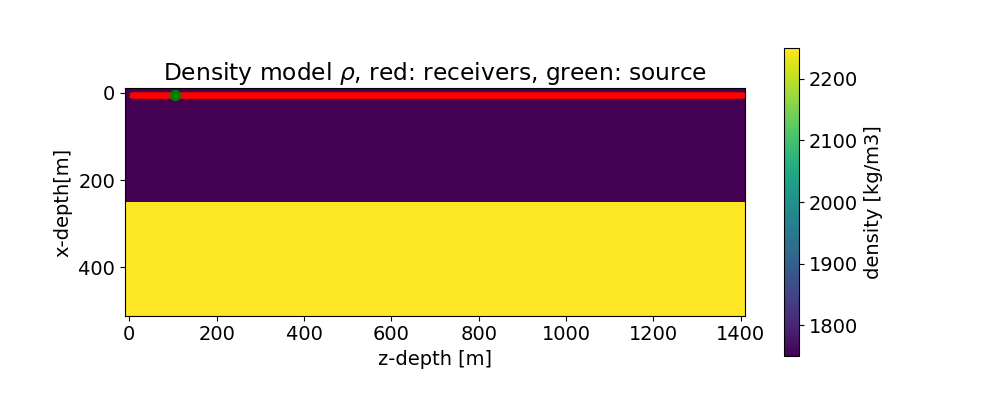
\includegraphics[width=\textwidth]{fig/rayleigh_model}
\caption{Earth model with 2 different materials. In the top layer $v_p$ =1800 (m/s), $v_s$ =1000 (m/s) and $\rho$ =1750 (kg/m3). In the bottom layer $v_p$ =3000 (m/s), $v_s$ =1500 (m/s) and $\rho$ =2250 (kg/m3).
}
\end{figure}
\clearpage
\begin{figure}[!h]\label{fig:rayleigh_shots}
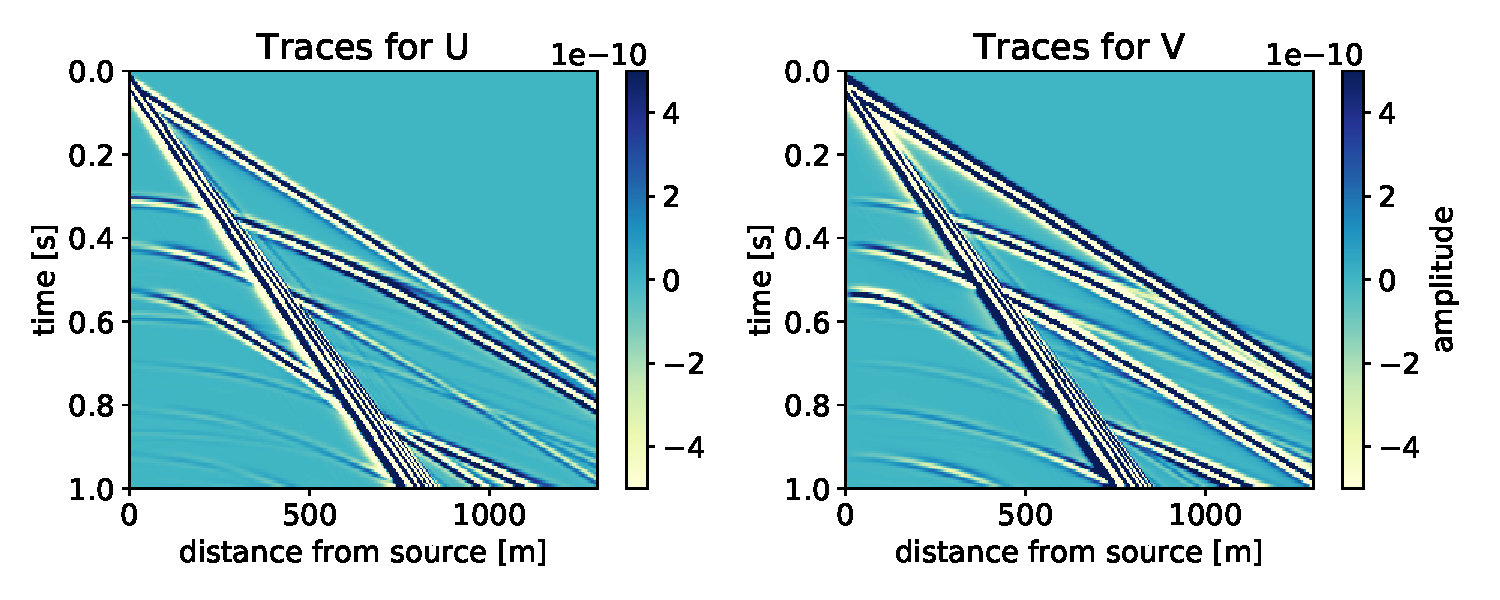
\includegraphics[width=\textwidth]{fig/rayleigh_shots.pdf}
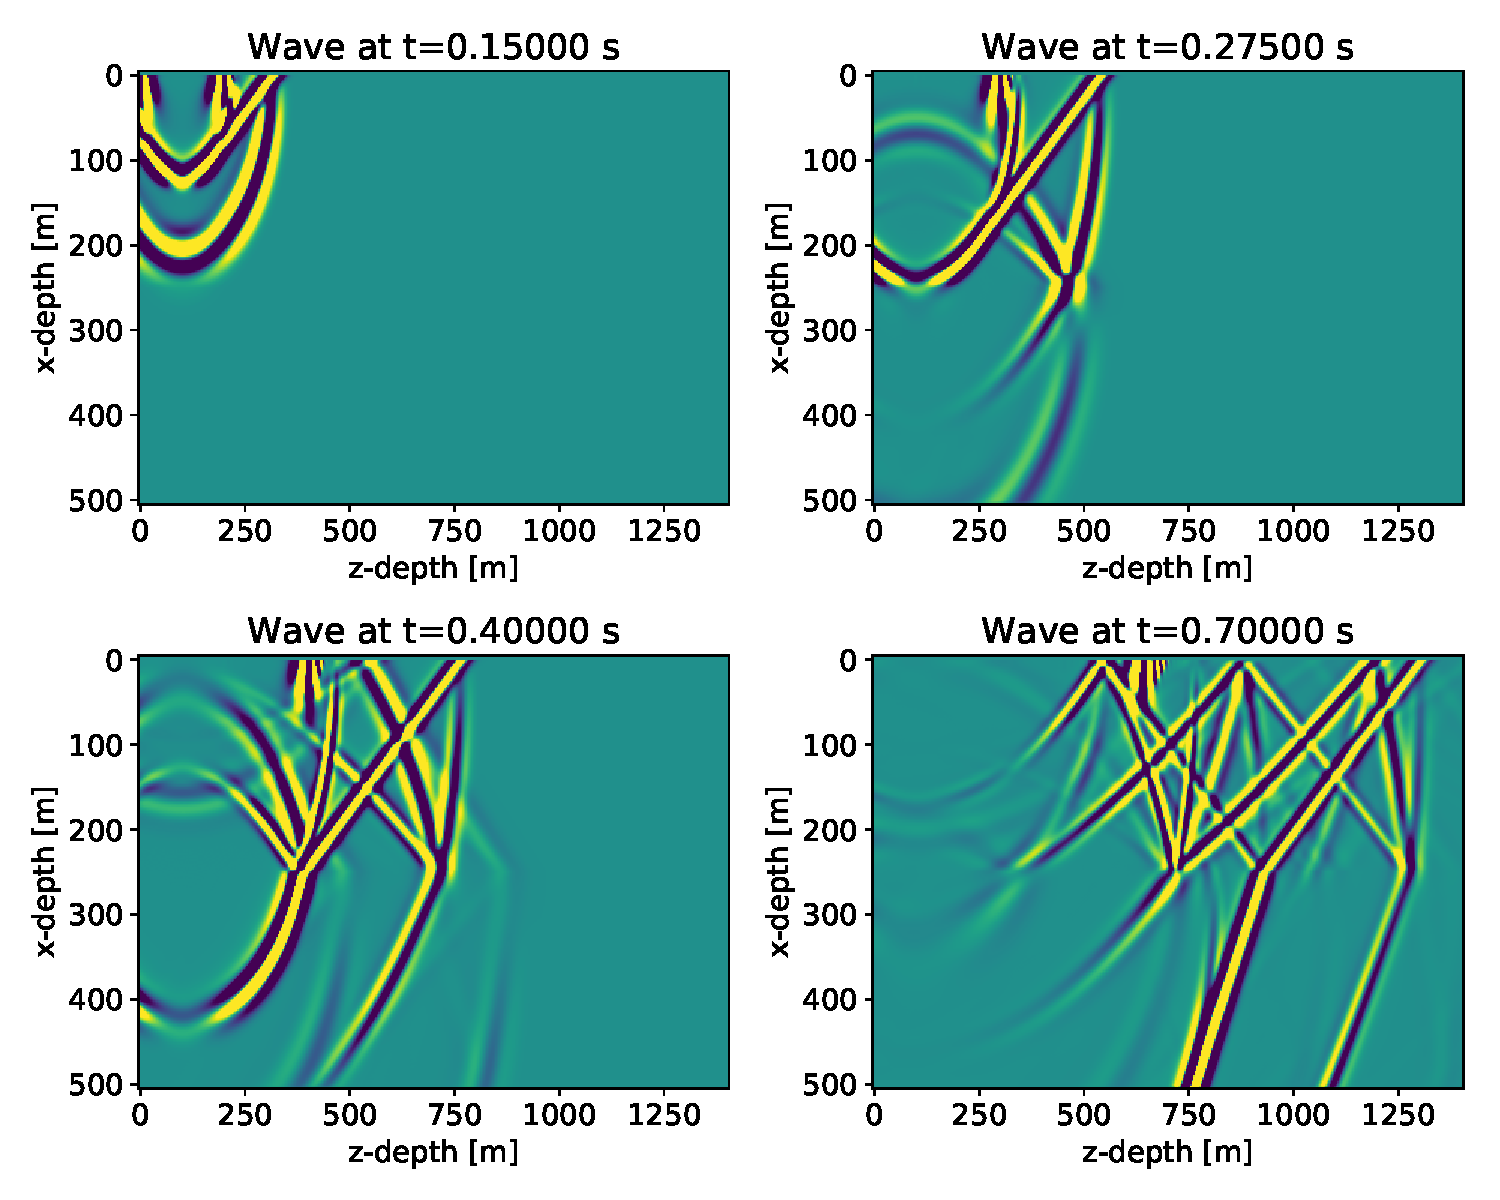
\includegraphics[width=0.93\textwidth]{fig/rayleigh_fields.pdf}
\caption{Free surface applied to the x=0 plane, top represent the shots and bottom four the $V_x$ field slices. Total grid format 2800 by 1000 points and 20000 timesteps, $dx=dz=0.5m$, $dt=0.05$ms, $f_q=30$Hz, CPML was applied on the other boundaries with standard settings(e.g 10 points, $R=0.001$).  }
\end{figure}
%----------------------------------------------------------------------------------------
%	REFERENCE LIST
%----------------------------------------------------------------------------------------
\phantomsection
\bibliographystyle{unsrt}
\bibliography{bib/UIS_ICP,custom}


%----------------------------------------------------------------------------------------

\end{document}